% Options for packages loaded elsewhere
\PassOptionsToPackage{unicode}{hyperref}
\PassOptionsToPackage{hyphens}{url}
%
\documentclass[
]{book}
\usepackage{amsmath,amssymb}
\usepackage{lmodern}
\usepackage{ifxetex,ifluatex}
\ifnum 0\ifxetex 1\fi\ifluatex 1\fi=0 % if pdftex
  \usepackage[T1]{fontenc}
  \usepackage[utf8]{inputenc}
  \usepackage{textcomp} % provide euro and other symbols
\else % if luatex or xetex
  \usepackage{unicode-math}
  \defaultfontfeatures{Scale=MatchLowercase}
  \defaultfontfeatures[\rmfamily]{Ligatures=TeX,Scale=1}
\fi
% Use upquote if available, for straight quotes in verbatim environments
\IfFileExists{upquote.sty}{\usepackage{upquote}}{}
\IfFileExists{microtype.sty}{% use microtype if available
  \usepackage[]{microtype}
  \UseMicrotypeSet[protrusion]{basicmath} % disable protrusion for tt fonts
}{}
\makeatletter
\@ifundefined{KOMAClassName}{% if non-KOMA class
  \IfFileExists{parskip.sty}{%
    \usepackage{parskip}
  }{% else
    \setlength{\parindent}{0pt}
    \setlength{\parskip}{6pt plus 2pt minus 1pt}}
}{% if KOMA class
  \KOMAoptions{parskip=half}}
\makeatother
\usepackage{xcolor}
\IfFileExists{xurl.sty}{\usepackage{xurl}}{} % add URL line breaks if available
\IfFileExists{bookmark.sty}{\usepackage{bookmark}}{\usepackage{hyperref}}
\hypersetup{
  pdftitle={Benjamin-Chung Lab Manual},
  hidelinks,
  pdfcreator={LaTeX via pandoc}}
\urlstyle{same} % disable monospaced font for URLs
\usepackage{color}
\usepackage{fancyvrb}
\newcommand{\VerbBar}{|}
\newcommand{\VERB}{\Verb[commandchars=\\\{\}]}
\DefineVerbatimEnvironment{Highlighting}{Verbatim}{commandchars=\\\{\}}
% Add ',fontsize=\small' for more characters per line
\usepackage{framed}
\definecolor{shadecolor}{RGB}{248,248,248}
\newenvironment{Shaded}{\begin{snugshade}}{\end{snugshade}}
\newcommand{\AlertTok}[1]{\textcolor[rgb]{0.94,0.16,0.16}{#1}}
\newcommand{\AnnotationTok}[1]{\textcolor[rgb]{0.56,0.35,0.01}{\textbf{\textit{#1}}}}
\newcommand{\AttributeTok}[1]{\textcolor[rgb]{0.77,0.63,0.00}{#1}}
\newcommand{\BaseNTok}[1]{\textcolor[rgb]{0.00,0.00,0.81}{#1}}
\newcommand{\BuiltInTok}[1]{#1}
\newcommand{\CharTok}[1]{\textcolor[rgb]{0.31,0.60,0.02}{#1}}
\newcommand{\CommentTok}[1]{\textcolor[rgb]{0.56,0.35,0.01}{\textit{#1}}}
\newcommand{\CommentVarTok}[1]{\textcolor[rgb]{0.56,0.35,0.01}{\textbf{\textit{#1}}}}
\newcommand{\ConstantTok}[1]{\textcolor[rgb]{0.00,0.00,0.00}{#1}}
\newcommand{\ControlFlowTok}[1]{\textcolor[rgb]{0.13,0.29,0.53}{\textbf{#1}}}
\newcommand{\DataTypeTok}[1]{\textcolor[rgb]{0.13,0.29,0.53}{#1}}
\newcommand{\DecValTok}[1]{\textcolor[rgb]{0.00,0.00,0.81}{#1}}
\newcommand{\DocumentationTok}[1]{\textcolor[rgb]{0.56,0.35,0.01}{\textbf{\textit{#1}}}}
\newcommand{\ErrorTok}[1]{\textcolor[rgb]{0.64,0.00,0.00}{\textbf{#1}}}
\newcommand{\ExtensionTok}[1]{#1}
\newcommand{\FloatTok}[1]{\textcolor[rgb]{0.00,0.00,0.81}{#1}}
\newcommand{\FunctionTok}[1]{\textcolor[rgb]{0.00,0.00,0.00}{#1}}
\newcommand{\ImportTok}[1]{#1}
\newcommand{\InformationTok}[1]{\textcolor[rgb]{0.56,0.35,0.01}{\textbf{\textit{#1}}}}
\newcommand{\KeywordTok}[1]{\textcolor[rgb]{0.13,0.29,0.53}{\textbf{#1}}}
\newcommand{\NormalTok}[1]{#1}
\newcommand{\OperatorTok}[1]{\textcolor[rgb]{0.81,0.36,0.00}{\textbf{#1}}}
\newcommand{\OtherTok}[1]{\textcolor[rgb]{0.56,0.35,0.01}{#1}}
\newcommand{\PreprocessorTok}[1]{\textcolor[rgb]{0.56,0.35,0.01}{\textit{#1}}}
\newcommand{\RegionMarkerTok}[1]{#1}
\newcommand{\SpecialCharTok}[1]{\textcolor[rgb]{0.00,0.00,0.00}{#1}}
\newcommand{\SpecialStringTok}[1]{\textcolor[rgb]{0.31,0.60,0.02}{#1}}
\newcommand{\StringTok}[1]{\textcolor[rgb]{0.31,0.60,0.02}{#1}}
\newcommand{\VariableTok}[1]{\textcolor[rgb]{0.00,0.00,0.00}{#1}}
\newcommand{\VerbatimStringTok}[1]{\textcolor[rgb]{0.31,0.60,0.02}{#1}}
\newcommand{\WarningTok}[1]{\textcolor[rgb]{0.56,0.35,0.01}{\textbf{\textit{#1}}}}
\usepackage{longtable,booktabs,array}
\usepackage{calc} % for calculating minipage widths
% Correct order of tables after \paragraph or \subparagraph
\usepackage{etoolbox}
\makeatletter
\patchcmd\longtable{\par}{\if@noskipsec\mbox{}\fi\par}{}{}
\makeatother
% Allow footnotes in longtable head/foot
\IfFileExists{footnotehyper.sty}{\usepackage{footnotehyper}}{\usepackage{footnote}}
\makesavenoteenv{longtable}
\usepackage{graphicx}
\makeatletter
\def\maxwidth{\ifdim\Gin@nat@width>\linewidth\linewidth\else\Gin@nat@width\fi}
\def\maxheight{\ifdim\Gin@nat@height>\textheight\textheight\else\Gin@nat@height\fi}
\makeatother
% Scale images if necessary, so that they will not overflow the page
% margins by default, and it is still possible to overwrite the defaults
% using explicit options in \includegraphics[width, height, ...]{}
\setkeys{Gin}{width=\maxwidth,height=\maxheight,keepaspectratio}
% Set default figure placement to htbp
\makeatletter
\def\fps@figure{htbp}
\makeatother
\setlength{\emergencystretch}{3em} % prevent overfull lines
\providecommand{\tightlist}{%
  \setlength{\itemsep}{0pt}\setlength{\parskip}{0pt}}
\setcounter{secnumdepth}{5}
\usepackage{booktabs}
\usepackage{amsthm}
\makeatletter
\def\thm@space@setup{%
  \thm@preskip=8pt plus 2pt minus 4pt
  \thm@postskip=\thm@preskip
}
\makeatother
\ifluatex
  \usepackage{selnolig}  % disable illegal ligatures
\fi
\usepackage[]{natbib}
\bibliographystyle{apalike}

\title{Benjamin-Chung Lab Manual}
\author{}
\date{\vspace{-2.5em}Updated: 2022-07-06}

\begin{document}
\maketitle

{
\setcounter{tocdepth}{1}
\tableofcontents
}
\hypertarget{welcome-to-the-benjamin-chung-lab}{%
\chapter{Welcome to the Benjamin-Chung Lab!}\label{welcome-to-the-benjamin-chung-lab}}

\hypertarget{about-the-lab}{%
\section{About the lab}\label{about-the-lab}}

Welcome to the lab of Dr.~Jade Benjamin-Chung, Assistant Professor in Epidemiology \& Population Health at Stanford University. Our mission is to improve population health by creating high quality evidence about what health interventions work in whom and where, when, and how to implement them. Most of our research is focused on infectious diseases, including malaria, diarrhea, soil-transmitted helminths, and influenza. Our focus is on improving the health of vulnerable populations from low-resource settings, both domestically and internationally. We use a variety of epidemiologic, computational, and statistical methods, including causal inference and machine learning methods, in pursuit of our mission. To learn more about the lab, visit \href{https://jadebc.net}{jadebc.net}.

\hypertarget{about-this-lab-manual}{%
\section{About this lab manual}\label{about-this-lab-manual}}

This lab manual covers our communication strategy, code of conduct, and best practices for reproducibility of computational workflows. It is a living document that is updated regularly.

This manual was created with input from a large number of team members and with inspiration from \href{https://github.com/alylab/labmanual/blob/master/aly-lab-manual.pdf}{other scientists' lab manuals}.
Contributors include Jade Benjamin-Chung, Kunal Mishra, Stephanie Djajadi, Nolan Pokpongkiat, and Anna Nguyen.

Feel free to draw from this manual (and please cite it if you do!).

This work is licensed under a Creative Commons Attribution-NonCommercial 4.0 International License.

\hypertarget{culture-and-conduct}{%
\chapter{Culture and conduct}\label{culture-and-conduct}}

by Jade Benjamin-Chung

\hypertarget{lab-culture}{%
\section{Lab culture}\label{lab-culture}}

We are committed to a lab culture that is collaborative, supportive, inclusive, open, and free from discrimination and harassment.

We encourage students / staff of all experience levels to respectfully share their honest opinions and ideas on any topic. Our group has thrived upon such respectful honest input from team members over the years, and this document is a product of years of student and staff input (and even debate) that has gradually improved our productivity and overall quality of our work.

\hypertarget{diversity-equity-and-inclusion}{%
\section{Diversity, equity, and inclusion}\label{diversity-equity-and-inclusion}}

The Benjamin-Chung lab recognizes the importance of and is committed to cultivating a culture of diversity, equity, and inclusion. This means being a safe, supportive, and anti-racist environment in which students from diverse backgrounds are equally and inclusively supported in their education and training. Diversity takes many forms, and includes, but is not limited to, differences in race, ethnicity, gender, sexuality, socioeconomic status, religion, disability, and political affiliation.

\hypertarget{protecting-human-subjects}{%
\section{Protecting human subjects}\label{protecting-human-subjects}}

All lab members must complete \href{https://researchcompliance.stanford.edu/panels/hs/forms/training/citi}{CITI Human Subjects Biomedical Group 1} training and share their certificate with Jade. She will add team members to relevant Institutional Review Board protocols prior to their start date to ensure they have permission to work with identifiable datasets.

One of the most relevant aspects of protecting human subjects in our work is maintaining confidentiality. For students supporting our data science efforts, in practice this means:

\begin{itemize}
\tightlist
\item
  Be sure to understand and comply with project-specific policies about where data can be saved, particularly if the data include personal identifiers.
\item
  Do not share data with anyone without permission, including to other members of the group, who might not be on the same IRB protocol as you (check with Jade first).
\end{itemize}

Remember, data that looks like it does not contain identifiers to you might still be classified as data that requires special protection by our IRB or under HIPAA, so always proceed with caution and ask for help if you have any concerns about how to maintain study participant confidentiality.

\hypertarget{authorship}{%
\section{Authorship}\label{authorship}}

We adhere to the \href{http://www.icmje.org/recommendations/browse/roles-and-responsibilities/defining-the-role-of-authors-and-contributors.html}{ICMJE Definition of authorship} and are happy for team members who meet the definition of authorship to be included as co-authors on scientific manuscripts.

\hypertarget{communication-and-coordination}{%
\chapter{Communication and coordination}\label{communication-and-coordination}}

by Jade Benjamin-Chung

One benefit of the academic environment is its schedule flexibility. This means that lab members may choose to work in the early morning, evening, or weekends. That said, we do not expect lab members to respond outside of business hours (unless there are special circumstances).

\hypertarget{slack}{%
\section{Slack}\label{slack}}

\begin{itemize}
\tightlist
\item
  Use Slack for scheduling, coding related questions, quick check ins, etc. If your Slack message exceeds 200 words, it might be time to use email.
\item
  Use channels instead of direct messages unless you need to discuss something private.
\item
  Please make an effort to respond to messages that message you (e.g., \texttt{@jade}) as quickly as possible and always within 24 hours.
\item
  If you are unusually busy (e.g., taking MCAT/GRE, taking many exams) or on vacation please alert the team in advance so we can expect you not to respond at all / as quickly as usual and also \href{https://get.slack.help/hc/en-us/articles/201864558-Set-your-Slack-status-and-availability}{set your status in Slack} (e.g., it could say ``On vacation'') so we know not to expect to see you online.
\item
  Please thread messages in Slack as much as possible.
\end{itemize}

\hypertarget{email}{%
\section{Email}\label{email}}

\begin{itemize}
\tightlist
\item
  Use email for longer messages (\textgreater200 words) or messages that merit preservation.
\item
  Generally, strive to respond within 24 hours hours. As noted above, if you are unusually busy or on vacation please alert the team in advance so we can expect you not to respond at all / as quickly as usual.
\end{itemize}

\hypertarget{trello}{%
\section{Trello}\label{trello}}

\begin{itemize}
\tightlist
\item
  Jade will add new cards within our shared Trello board that outline your tasks.
\item
  The higher a card is within your list, the higher priority it is.
\item
  Generally, strive to complete the tasks in your card by the date listed.
\item
  Use checklists to break down a task into smaller chunks. Sometimes Jade will write this for you, but you can also add this yourself.
\item
  Jade will move your card to the ``Completed'' list when it is done.
\end{itemize}

\hypertarget{google-drives}{%
\section{Google Drives}\label{google-drives}}

\begin{itemize}
\tightlist
\item
  We mostly use Google Drive to create shared documents with longer descriptions of tasks. These documents are linked to in Trello. Jade often shares these with the whole team since tasks are overlapping, and even if a task is assigned to one person, others may have valuable insights.
\end{itemize}

\hypertarget{meetings}{%
\section{Meetings}\label{meetings}}

\begin{itemize}
\tightlist
\item
  Our meetings start on the hour.
\item
  If you are going to be late, please send a message in our Slack channel.
\item
  If you are regularly not able to come on the hour, notify the team and we might choose the modify the agenda order or the start time.
\end{itemize}

\hypertarget{reproducibility}{%
\chapter{Reproducibility}\label{reproducibility}}

by Jade Benjamin-Chung

Our lab adopts the following practices to maximize the reproducibility of our work.

\begin{enumerate}
\def\labelenumi{\arabic{enumi}.}
\tightlist
\item
  Design studies with appropriate methodology and adherence to best practices in epidemiology and biostatistics
\item
  Register study protocols
\item
  Write and register pre-analysis plans
\item
  Create reproducible workflows
\item
  Process and analyze data with internal replication and masking
\item
  Use reporting checklists with manuscripts
\item
  Publish preprints
\item
  Publish data (when possible) and replication scripts
\end{enumerate}

\hypertarget{what-is-the-reproducibility-crisis}{%
\section{What is the reproducibility crisis?}\label{what-is-the-reproducibility-crisis}}

In the past decade, an increasing number of studies have found that published study findings could not be reproduced. Researchers found that it was not possible to reproduce estimates from published studies: 1) with the same data and same or similar code and 2) with newly collected data using the same (or similar) study design. These ``failures'' of reproducibility were frequent enough and broad enough in scope, occurring across a range of disciplines (epidemiology, psychology, economics, and others) to be deeply troubling. Program and policy decisions based on erroneous research findings could lead to wasted resources, and at worst, could harm intended beneficiaries. This crisis has motivated new practices in reproducibility, transparency, and openness. Our lab is committed to adopting these best practices, and much of the remainder of the lab manual focuses on how to do so.

Recommended readings on the ``reproducibility crisis'':

\begin{itemize}
\item
  Nuzzo R. How scientists fool themselves -- and how they can stop. 2015. \href{}{https://www.nature.com/articles/526182a}
\item
  Stoddart C. Is there a reproducibility crisis in science? 2016. \url{https://www.nature.com/articles/d41586-019-00067-3}
\item
  Munafo MR, et al.~A manifesto for reproducible science. \emph{Nature Human Behavior} 2017 \url{http://dx.doi.org/10.1038/s41562-016-0021}
\end{itemize}

\hypertarget{study-design}{%
\section{Study design}\label{study-design}}

Appropriate study design is beyond the scope of this lab manual and is something trainees develop through their coursework and mentoring.

\hypertarget{register-study-protocols}{%
\section{Register study protocols}\label{register-study-protocols}}

We register all randomized trials on \url{clinicaltrials.gov}, and in some cases register observational studies as well.

\hypertarget{write-and-register-pre-analysis-plans}{%
\section{Write and register pre-analysis plans}\label{write-and-register-pre-analysis-plans}}

We write pre-analysis plans for most original research projects that are not exploratory in nature, although in some cases, we write pre-analysis plans for exploratory studies as well. The format and content of pre-analysis plans can vary from project to project. Here is an example of one: \url{https://osf.io/tgbxr/}. Generally, these include:

\begin{enumerate}
\def\labelenumi{\arabic{enumi}.}
\tightlist
\item
  Brief background on the study (a condensed version of the introduction section of the paper)
\item
  Hypotheses / objectives
\item
  Study design
\item
  Description of data
\item
  Definition of outcomes
\item
  Definition of interventions / exposures
\item
  Definition of covariates
\item
  Statistical power calculation
\item
  Statistical analysis:
\end{enumerate}

\begin{itemize}
\tightlist
\item
  Type of model
\item
  Covariate selection / screening
\item
  Standard error estimation method
\item
  Missing data analysis
\item
  Assessment of effect modification / subgroup analyses
\item
  Sensitivity analyses
\item
  Negative control analyses
\end{itemize}

\hypertarget{create-reproducible-workflows}{%
\section{Create reproducible workflows}\label{create-reproducible-workflows}}

Reproducible workflows allow a user to reproduce study estimates and ideally figures and tables with a ``single click''. In practice, this typically means running a single bash script that sources all replication scripts in a repository. These replication scripts complete data processing, data analysis, and figure/table generation. The following chapters provide detailed guidance on this topic:

\begin{itemize}
\tightlist
\item
  Chapter 5: Code repositories
\item
  Chapter 6: Coding practices
\item
  Chapter 7: Coding style
\item
  Chapter 8: Code publication
\item
  Chapter 9: Working with big data
\item
  Chapter 10: Github
\item
  Chapter 11: Unix
\end{itemize}

\hypertarget{process-and-analyze-data-with-internal-replication-and-masking}{%
\section{Process and analyze data with internal replication and masking}\label{process-and-analyze-data-with-internal-replication-and-masking}}

See my video on this topic: \url{https://www.youtube.com/watch?v=WoYkY9MkbRE}

\hypertarget{use-reporting-checklists-with-manuscripts}{%
\section{Use reporting checklists with manuscripts}\label{use-reporting-checklists-with-manuscripts}}

Using reporting checklists helps ensure that peer-reviewed articles contain the information needed for readers to assess the validity of your work and/or attempt to reproduce it. A collection of reporting checklists is available here: \href{https://www.equator-network.org/about-us/what-is-a-reporting-guideline/}{https://www.equator-network.org/about-us/what-is-a-reporting-guideline/)}

\hypertarget{publish-preprints}{%
\section{Publish preprints}\label{publish-preprints}}

A preprint is a scientific manuscript that has not been peer reviewed. Preprint servers create digital object identifiers (DOIs) and can be cited in other articles and in grant applications. Because the peer review process can take many months, publishing preprints prior to or during peer review enables other scientists to immediately learn from and build on your work. Importantly, NIH allows applicants to include preprint citations in their biosketches. In most cases, we publish preprints on \href{https://www.medrxiv.org/}{medRxiv}.

\hypertarget{publish-data-when-possible-and-replication-scripts}{%
\section{Publish data (when possible) and replication scripts}\label{publish-data-when-possible-and-replication-scripts}}

Publishing data and replication scripts allows other scientists to reproduce your work and to build upon it. We typically publish data on \href{osf.io}{Open Science Framework}, share links to \href{github.com}{Github} repositories, and archive code on \href{zenodo.org}{Zenodo}.

\hypertarget{code-repositories}{%
\chapter{Code repositories}\label{code-repositories}}

By Kunal Mishra, Jade Benjamin-Chung, and Stephanie Djajadi

Each study has at least one code repository that typically holds R code, shell scripts with Unix code, and research outputs (results .RDS files, tables, figures). Repositories may also include datasets. This chapter outlines how to organize these files. Adhering to a standard format makes it easier for us to efficiently collaborate across projects.

\hypertarget{project-structure}{%
\section{Project Structure}\label{project-structure}}

We recommend the following directory structure:

\begin{verbatim}
0-run-project.sh
0-config.R
1 - Data-Management/
    0-prep-data.sh
    1-prep-cdph-fluseas.R
    2a-prep-absentee.R
    2b-prep-absentee-weighted.R
    3a-prep-absentee-adj.R
    3b-prep-absentee-adj-weighted.R
2 - Analysis/
    0-run-analysis.sh
    1 - Absentee-Mean/
        1-absentee-mean-primary.R
        2-absentee-mean-negative-control.R
        3-absentee-mean-CDC.R
        4-absentee-mean-peakwk.R
        5-absentee-mean-cdph2.R
        6-absentee-mean-cdph3.R
    2 - Absentee-Positivity-Check/
    3 - Absentee-P1/
    4 - Absentee-P2/
3 - Figures/
    0-run-figures.sh
    ...
4 - Tables/
    0-run-tables.sh
    ...
5 - Results/
    1 - Absentee-Mean/
        1-absentee-mean-primary.RDS
        2-absentee-mean-negative-control.RDS
        3-absentee-mean-CDC.RDS
        4-absentee-mean-peakwk.RDS
        5-absentee-mean-cdph2.RDS
        6-absentee-mean-cdph3.RDS
    ...
.gitignore
.Rproj
\end{verbatim}

For brevity, not every directory is ``expanded'', but we can glean some important takeaways from what we \emph{do} see.

\hypertarget{rproj-files}{%
\section{\texorpdfstring{\texttt{.Rproj} files}{.Rproj files}}\label{rproj-files}}

An ``R Project'' can be created within RStudio by going to \texttt{File\ \textgreater{}\textgreater{}\ New\ Project}. Depending on where you are with your research, choose the most appropriate option. This will save preferences, working directories, and even the results of running code/data (though I'd recommend starting from scratch each time you open your project, in general). Then, ensure that whenever you are working on that specific research project, you open your created project to enable the full utility of \texttt{.Rproj} files. This also automatically sets the directory to the top level of the project.

\hypertarget{configuration-config-file}{%
\section{Configuration (`config') File}\label{configuration-config-file}}

This is the single most important file for your project. It will be responsible for a variety of common tasks, declare global variables, load functions, declare paths, and more. \emph{Every other file in the project} will begin with \texttt{source("0-config")}, and its role is to reduce redundancy and create an abstraction layer that allows you to make changes in one place (\texttt{0-config.R}) rather than 5 different files. To this end, paths which will be reference in multiple scripts (i.e.~a \texttt{merged\_data\_path}) can be declared in \texttt{0-config.R} and simply referred to by its variable name in scripts. If you ever want to change things, rename them, or even switch from a downsample to the full data, all you would then to need to do is modify the path in one place and the change will automatically update throughout your project. See the example config file for more details. The paths defined in the \texttt{0-config.R} file assume that users have opened the \texttt{.Rproj} file, which sets the directory to the top level of the project.

\hypertarget{order-files-and-directories}{%
\section{Order Files and Directories}\label{order-files-and-directories}}

This makes the jumble of alphabetized filenames much more coherent and places similar code and files next to one another. This also helps us understand how data flows from start to finish and allows us to easily map a script to its output (i.e.~\texttt{2\ -\ Analysis/1\ -\ Absentee-Mean/1-absentee-mean-primary.R} =\textgreater{} \texttt{5\ -\ Results/1\ -\ Absentee-Mean/1-absentee-mean-primary.RDS}). If you take nothing else away from this guide, this is the single most helpful suggestion to make your workflow more coherent. Often the particular order of files will be in flux until an analysis is close to completion. At that time it is important to review file order and naming and reproduce everything prior to drafting a manuscript.

\hypertarget{using-bash-scripts-to-ensure-reproducibility}{%
\section{Using Bash scripts to ensure reproducibility}\label{using-bash-scripts-to-ensure-reproducibility}}

Bash scripts are useful components of a reproducible workflow. At many of the directory levels (i.e.~in \texttt{3\ -\ Analysis}), there is a bash script that runs each of the analysis scripts. This is exceptionally useful when data ``upstream'' changes -- you simply run the bash script. See the \protect\hyperlink{unix}{Unix Chapter} for further details.

After running bash scripts, \texttt{.Rout} log files will be generated for each script that has been executed. It is important to check these files. Scripts may appear to have run correctly in the terminal, but checking the log files is the only way to ensure that everything has run completely.

\hypertarget{coding-practices}{%
\chapter{Coding practices}\label{coding-practices}}

by Kunal Mishra, Jade Benjamin-Chung, and Stephanie Djajadi

\hypertarget{organizing-scripts}{%
\section{Organizing scripts}\label{organizing-scripts}}

Just as your data ``flows'' through your project, data should flow naturally through a script. Very generally, you want to:

\begin{enumerate}
\def\labelenumi{\arabic{enumi}.}
\tightlist
\item
  describe the work completed in the script in a comment header
\item
  source your configuration file (\texttt{0-config.R})
\item
  load all your data
\item
  do all your analysis/computation
\item
  save your data.
\end{enumerate}

Each of these sections should be ``chunked together'' using comments. See \href{https://github.com/kmishra9/Flu-Absenteeism/blob/master/Master's\%20Thesis\%20-\%20Spatial\%20Epidemiology\%20of\%20Influenza/2a\%20-\%20Statistical-Inputs.R}{this file} for a good example of how to cleanly organize a file in a way that follows this ``flow'' and functionally separate pieces of code that are doing different things.

\hypertarget{documenting-your-code}{%
\section{Documenting your code}\label{documenting-your-code}}

\hypertarget{file-headers}{%
\subsection{File headers}\label{file-headers}}

Every file in a project should have a header that allows it to be interpreted on its own. It should include the name of the project and a short description for what this file (among the many in your project) does specifically. You may optionally wish to include the inputs and outputs of the script as well, though the next section makes this significantly less necessary.

\begin{verbatim}
################################################################################
# @Organization - Example Organization
# @Project - Example Project
# @Description - This file is responsible for [...]
################################################################################
\end{verbatim}

\hypertarget{sections-and-subsections}{%
\subsection{Sections and subsections}\label{sections-and-subsections}}

Rstudio (\href{https://blog.rstudio.com/2020/12/02/rstudio-v1-4-preview-little-things/}{v1.4 or more recent}) supports the use of Sections and Subsections. You can easily navigate through longer scripts using the navigation pane in RStudio, as shown on the right below.

\begin{verbatim}
# Section -------

## Subsection -------

### Sub-subsection -------
\end{verbatim}

\hypertarget{code-folding}{%
\subsection{Code folding}\label{code-folding}}

Consider using RStudio's \href{https://support.rstudio.com/hc/en-us/articles/200484568-Code-Folding-and-Sections}{code folding} feature to collapse and expand different sections of your code. Any comment line with at least four trailing dashes (-), equal signs (=), or pound signs (\#) automatically creates a code section. For example:

\hypertarget{comments-in-the-body-of-your-script}{%
\subsection{Comments in the body of your script}\label{comments-in-the-body-of-your-script}}

Commenting your code is an important part of reproducibility and helps document your code for the future. When things change or break, you'll be thankful for comments. There's no need to comment excessively or unnecessarily, but a comment describing what a large or complex chunk of code does is always helpful. See \href{https://github.com/kmishra9/Flu-Absenteeism/blob/master/Master's\%20Thesis\%20-\%20Spatial\%20Epidemiology\%20of\%20Influenza/1b\%20-\%20Map-Management.R}{this file} for an example of how to comment your code and notice that comments are always in the form of:

\texttt{\#\ This\ is\ a\ comment\ -\/-\ first\ letter\ is\ capitalized\ and\ spaced\ away\ from\ the\ pound\ sign}

\hypertarget{function-documentation}{%
\subsection{Function documentation}\label{function-documentation}}

Every function you write must include a header to document its purpose, inputs, and outputs. For any reproducible workflows, they are essential, because R is dynamically typed. This means, you can pass a \texttt{string} into an argument that is meant to be a \texttt{data.table}, or a \texttt{list} into an argument meant for a \texttt{tibble}. It is the responsibility of a function's author to document what each argument is meant to do and its basic type. This is an example for documenting a function (inspired by \href{https://www.oracle.com/technetwork/java/javase/documentation/index-137868.html\#format}{JavaDocs} and R's \href{https://blog.rstudio.com/2018/10/23/rstudio-1-2-preview-plumber-integration/}{Plumber API docs}):

\begin{verbatim}
##############################################
##############################################
# Documentation: calc_fluseas_mean
# Usage: calc_fluseas_mean(data, yname)
# Description: Make a dataframe with rows for flu season and site
# and the number of patients with an outcome, the total patients,
# and the percent of patients with the outcome

# Args/Options:
# data: a data frame with variables flu_season, site, studyID, and yname
# yname: a string for the outcome name
# silent: a boolean specifying whether the function shouldn't output anything to the console (DEFAULT: TRUE)

# Returns: the dataframe as described above
# Output: prints the data frame described above if silent is not True

calc_fluseas_mean = function(data, yname, silent = TRUE) {
 ### function code here 

}
\end{verbatim}

The header tells you what the function does, its various inputs, and how you might go about using the function to do what you want. Also notice that all optional arguments (i.e.~ones with pre-specified defaults) follow arguments that require user input.

\begin{itemize}
\item
  \textbf{Note}: As someone trying to call a function, it is possible to access a function's documentation (and internal code) by \texttt{CMD-Left-Click}ing the function's name in RStudio
\item
  \textbf{Note}: Depending on how important your function is, the complexity of your function code, and the complexity of different types of data in your project, you can also add ``type-checking'' to your function with the \texttt{assertthat::assert\_that()} function. You can, for example, \texttt{assert\_that(is.data.frame(statistical\_input))}, which will ensure that collaborators or reviewers of your project attempting to use your function are using it in the way that it is intended by calling it with (at the minimum) the correct type of arguments. You can extend this to ensure that certain assumptions regarding the inputs are fulfilled as well (i.e.~that \texttt{time\_column}, \texttt{location\_column}, \texttt{value\_column}, and \texttt{population\_column} all exist within the \texttt{statistical\_input} tibble).
\end{itemize}

\hypertarget{object-naming}{%
\section{Object naming}\label{object-naming}}

Generally we recommend using nouns for objects and verbs for functions. This is because functions are performing actions, while objects are not.

Try to make your variable names both more expressive and more explicit. Being a bit more verbose is useful and easy in the age of autocompletion! For example, instead of naming a variable \texttt{vaxcov\_1718}, try naming it \texttt{vaccination\_coverage\_2017\_18}. Similarly, \texttt{flu\_res} could be named \texttt{absentee\_flu\_residuals}, making your code more readable and explicit.

\begin{itemize}
\tightlist
\item
  For more help, check out \href{https://spin.atomicobject.com/2017/11/01/good-variable-names/}{Be Expressive: How to Give Your Variables Better Names}
\end{itemize}

We recommend you use \textbf{Snake\_Case}.

\begin{itemize}
\item
  Base R allows \texttt{.} in variable names and functions (such as \texttt{read.csv()}), but this goes against best practices for variable naming in many other coding languages. For consistency's sake, \texttt{snake\_case} has been adopted across languages, and modern packages and functions typically use it (i.e.~\texttt{readr::read\_csv()}). As a very general rule of thumb, if a package you're using doesn't use \texttt{snake\_case}, there may be an updated version or more modern package that \emph{does}, bringing with it the variety of performance improvements and bug fixes inherent in more mature and modern software.
\item
  \textbf{Note}: you may also see \texttt{camelCase} throughout the R code you come across. This is \emph{okay} but not ideal -- try to stay consistent across all your code with \texttt{snake\_case}.
\item
  \textbf{Note}: again, its also worth noting there's nothing inherently wrong with using \texttt{.} in variable names, just that it goes against style best practices that are cropping up in data science, so its worth getting rid of these bad habits now.
\end{itemize}

\hypertarget{function-calls}{%
\section{Function calls}\label{function-calls}}

In a function call, use ``named arguments'' and put each argument on a separate line to make your code more readable.

Here's an example of what not to do when calling the function a function \texttt{calc\_fluseas\_mean} (defined above):

\begin{verbatim}
mean_Y = calc_fluseas_mean(flu_data, "maari_yn", FALSE)
\end{verbatim}

And here it is again using the best practices we've outlined:

\begin{verbatim}
mean_Y = calc_fluseas_mean(
  data = flu_data, 
  yname = "maari_yn",
  silent = FALSE
)
\end{verbatim}

\hypertarget{the-here-package}{%
\section{The here package}\label{the-here-package}}

The \texttt{here} package is one great R package that helps multiple collaborators deal with the mess that is working directories within an R project structure. Let's say we have an R project at the path \texttt{/home/oski/Some-R-Project}. My collaborator might clone the repository and work with it at some other path, such as \texttt{/home/bear/R-Code/Some-R-Project}. Dealing with working directories and paths explicitly can be a very large pain, and as you might imagine, setting up a Config with paths requires those paths to flexibly work for all contributors to a project. This is where the \texttt{here} package comes in and this a \href{https://github.com/jennybc/here_here}{great vignette describing it}.

\hypertarget{readingsaving-data}{%
\section{Reading/Saving Data}\label{readingsaving-data}}

\hypertarget{rds-vs-.rdata-files}{%
\subsection{\texorpdfstring{\texttt{.RDS} vs \texttt{.RData} Files}{.RDS vs .RData Files}}\label{rds-vs-.rdata-files}}

One of the most common ways to load and save data in Base R is with the \texttt{load()} and \texttt{save()} functions to serialize multiple objects in a single \texttt{.RData} file. The biggest problems with this practice include an inability to control the names of things getting loaded in, the inherent confusion this creates in understanding older code, and the inability to load individual elements of a saved file. For this, we recommend using the RDS format to save R objects.

\begin{itemize}
\tightlist
\item
  \textbf{Note}: if you have many related R objects you would have otherwise saved all together using the \texttt{save} function, the functional equivalent with \texttt{RDS} would be to create a (named) list containing each of these objects, and saving it.
\end{itemize}

\hypertarget{csvs}{%
\subsection{CSVs}\label{csvs}}

Once again, the \texttt{readr} package as part of the Tidvyerse is great, with a much faster \texttt{read\_csv()} than Base R's \texttt{read.csv()}. For massive CSVs (\textgreater{} 5 GB), you'll find \texttt{data.table::fread()} to be the fastest CSV reader in any data science language out there. For writing CSVs, \texttt{readr::write\_csv()} and \texttt{data.table::fwrite()} outclass Base R's \texttt{write.csv()} by a significant margin as well.

\hypertarget{integrating-box-and-dropbox}{%
\section{Integrating Box and Dropbox}\label{integrating-box-and-dropbox}}

Box and Dropbox are cloud-based file sharing systems that are useful when dealing with large files. When our scripts generate large output files, the files can slow down the workflow if they are pushed to GitHub. This makes collaboration difficult when not everyone has a copy of the file, unless we decide to duplicate files and share them manually. The files might also take up a lot of local storage. Box and Dropbox help us avoid these issues by automatically storing the files, reading data, and writing data back to the cloud.

Box and Dropbox are separate platforms, but we can use either one to store and share files. To use them, we can install the packages that have been created to integrate Box and Dropbox into R. The set-up instructions are detailed below.

Make sure to authenticate before reading and writing from either Box or Dropbox. The authentication commands should go in the configuration file; it only needs to be done once. This will prompt you to give your login credentials for Box and Dropbox and will allow your application to access your shared folders.

\hypertarget{box}{%
\subsection{Box}\label{box}}

Follow the instructions in this section to use the \texttt{boxr} package. Note that there are a few setup steps that need to be done on the box website before you can use the \texttt{boxr} package, \href{https://r-box.github.io/boxr/articles/boxr-app-interactive.html\#create}{explained here} in the section ``Creating an Interactive App.'' This gets the authentication keys that must be put in box.
Once that is done, add the authentication keys to your code in the configuration file, with \texttt{box\_auth(client\_id\ =\ "\textless{}your\_client\_id\textgreater{}",\ client\_secret\ =\ "\textless{}your\_client\_secret\_id\textgreater{}")}. It is also important to set the default working directory so that the code can reference the correct folder in box: \texttt{box\_setwd(\textless{}folder\_id\textgreater{})}. The folder ID is the sequence of digits at the end of the URL.

Further details can be found \href{https://github.com/r-box/boxr}{here}.

\hypertarget{dropbox}{%
\subsection{Dropbox}\label{dropbox}}

Follow the instructions at \href{https://github.com/karthik/rdrop2}{this link} to use the \texttt{rdrop2} package. Similar to the \texttt{boxr} package, you must authenticate before reading and writing from Dropbox, which can be done by adding \texttt{drop\_auth()} to the configuration file.

Saving the authentication token is not required, although it may be useful if you plan on using Dropbox frequently. To do so, save the token with the following commands. Tokens are valid until they are manually revoked.

\begin{verbatim}
# first time only
# save the output of drop_auth to an RDS file
token <- drop_auth()
# this token only has to be generated once, it is valid until revoked
saveRDS(token, "/path/to/tokenfile.RDS")

# all future usages
# to use a stored token, provide the rdstoken argument
drop_auth(rdstoken = "/path/to/tokenfile.RDS")
\end{verbatim}

\hypertarget{tidyverse}{%
\section{Tidyverse}\label{tidyverse}}

Throughout this document there have been references to the Tidyverse, but this section is to explicitly show you how to transform your Base R tendencies to Tidyverse (or Data.Table, Tidyverse's performance-optimized competitor). For most of our work that does not utilize very large datasets, we recommend that you code in Tidyverse rather than Base R. Tidyverse is quickly becoming \href{https://rviews.rstudio.com/2017/06/08/what-is-the-tidyverse/}{the gold standard} in R data analysis and modern data science packages and code should use Tidyverse style and packages unless there's a significant reason not to (i.e.~big data pipelines that would benefit from Data.Table's performance optimizations).

The package author has published a \href{https://r4ds.had.co.nz/}{great textbook on R for Data Science}, which leans heavily on many Tidyverse packages and may be worth checking out.

The following list is not exhaustive, but is a compact overview to begin to translate Base R into something better:

\begin{longtable}[]{@{}
  >{\raggedright\arraybackslash}p{(\columnwidth - 2\tabcolsep) * \real{0.50}}
  >{\raggedright\arraybackslash}p{(\columnwidth - 2\tabcolsep) * \real{0.50}}@{}}
\toprule
Base R & Better Style, Performance, and Utility \\
\midrule
\endhead
\_ & \_ \\
\texttt{read.csv()} & \texttt{readr::read\_csv()} or \texttt{data.table::fread()} \\
\texttt{write.csv()} & \texttt{readr::write\_csv()} or \texttt{data.table::fwrite()} \\
\texttt{readRDS} & \texttt{readr::read\_rds()} \\
\texttt{saveRDS()} & \texttt{readr::write\_rds()} \\
\_ & \_ \\
\texttt{data.frame()} & \texttt{tibble::tibble()} or \texttt{data.table::data.table()} \\
\texttt{rbind()} & \texttt{dplyr::bind\_rows()} \\
\texttt{cbind()} & \texttt{dplyr::bind\_cols()} \\
\texttt{df\$some\_column} & \texttt{df\ \%\textgreater{}\%\ dplyr::pull(some\_column)} \\
\texttt{df\$some\_column\ =\ ...} & \texttt{df\ \%\textgreater{}\%\ dplyr::mutate(some\_column\ =\ ...)} \\
\texttt{df{[}get\_rows\_condition,{]}} & \texttt{df\ \%\textgreater{}\%\ dplyr::filter(get\_rows\_condition)} \\
\texttt{df{[},c(col1,\ col2){]}} & \texttt{df\ \%\textgreater{}\%\ dplyr::select(col1,\ col2)} \\
\texttt{merge(df1,\ df2,\ by\ =\ ...,\ all.x\ =\ ...,\ all.y\ =\ ...)} & \texttt{df1\ \%\textgreater{}\%\ dplyr::left\_join(df2,\ by\ =\ ...)} or \texttt{dplyr::full\_join} or \texttt{dplyr::inner\_join} or \texttt{dplyr::right\_join} \\
\_ & \_ \\
\texttt{str()} & \texttt{dplyr::glimpse()} \\
\texttt{grep(pattern,\ x)} & \texttt{stringr::str\_which(string,\ pattern)} \\
\texttt{gsub(pattern,\ replacement,\ x)} & \texttt{stringr::str\_replace(string,\ pattern,\ replacement)} \\
\texttt{ifelse(test\_expression,\ yes,\ no)} & \texttt{if\_else(condition,\ true,\ false)} \\
Nested: \texttt{ifelse(test\_expression1,\ yes1,\ ifelse(test\_expression2,\ yes2,\ ifelse(test\_expression3,\ yes3,\ no)))} & \texttt{case\_when(test\_expression1\ \textasciitilde{}\ yes1,\ \ test\_expression2\ \textasciitilde{}\ yes2,\ test\_expression3\ \textasciitilde{}\ yes3,\ TRUE\ \textasciitilde{}\ no)} \\
\texttt{proc.time()} & \texttt{tictoc::tic()} and \texttt{tictoc::toc()} \\
\texttt{stopifnot()} & \texttt{assertthat::assert\_that()} or \texttt{assertthat::see\_if()} or \texttt{assertthat::validate\_that()} \\
\bottomrule
\end{longtable}

For a more extensive set of syntactical translations to Tidyverse, you can check out \href{https://tavareshugo.github.io/data_carpentry_extras/base-r_tidyverse_equivalents/base-r_tidyverse_equivalents.html\#reshaping_data}{this document}.

Working with Tidyverse within functions can be somewhat of a pain due to non-standard evaluation (NSE) semantics. If you're an avid function writer, we'd recommend checking out the following resources:

\begin{itemize}
\tightlist
\item
  \href{https://www.youtube.com/watch?v=nERXS3ssntw}{Tidy Eval in 5 Minutes} (video)
\item
  \href{https://tidyeval.tidyverse.org/index.html}{Tidy Evaluation} (e-book)
\item
  \href{https://www.brodrigues.co/blog/2016-07-18-data-frame-columns-as-arguments-to-dplyr-functions/}{Data Frame Columns as Arguments to Dplyr Functions} (blog)
\item
  \href{https://stackoverflow.com/questions/28125816/r-standard-evaluation-for-join-dplyr}{Standard Evaluation for *\_join} (stackoverflow)
\item
  \href{https://dplyr.tidyverse.org/articles/programming.html}{Programming with dplyr} (package vignette)
\end{itemize}

\hypertarget{coding-with-r-and-python}{%
\section{Coding with R and Python}\label{coding-with-r-and-python}}

If you're using both R and Python, you may wish to check out the \href{https://www.rdocumentation.org/packages/feather/versions/0.3.3}{Feather package} for exchanging data between the two languages \href{https://blog.rstudio.com/2016/03/29/feather/}{extremely quickly}.

\hypertarget{reviewing-code}{%
\section{Reviewing Code}\label{reviewing-code}}

Before publishing new changes, it is important to ensure that the code has been tested and well-documented. GitHub makes it possible to document all of these changes in a pull request. Pull requests can be used to describe changes in a branch that are ready to be merged with the base branch (more information in the \protect\hyperlink{Github}{GitHub} section). Github allows users to create a pull request template in a repository to standardize and customize the information in a pull request. When you add a pull request template to your repository, everyone will automatically see the template's contents in the pull request body.

\hypertarget{creating-a-pull-request-template}{%
\subsection{Creating a Pull Request Template}\label{creating-a-pull-request-template}}

Follow the instructions below to add a pull request template to a repository. More details can be found at this \href{https://help.github.com/en/github/building-a-strong-community/creating-a-pull-request-template-for-your-repository}{GitHub link}.

\begin{enumerate}
\def\labelenumi{\arabic{enumi}.}
\tightlist
\item
  On GitHub, navigate to the main page of the repository.
\item
  Above the file list, click \texttt{Create\ new\ file}.
\item
  Name the file \texttt{pull\_request\_template.md}. GitHub will not recognize this as the template if it is named anything else. The file must be on the \texttt{master} branch.

  \begin{enumerate}
  \def\labelenumii{\arabic{enumii}.}
  \tightlist
  \item
    To store the file in a hidden directory instead of the main directory, name the file \texttt{.github/pull\_request\_template.md}.
  \end{enumerate}
\item
  In the body of the new file, add your pull request template. This could include:

  \begin{itemize}
  \tightlist
  \item
    A summary of the changes proposed in the pull request
  \item
    How the change has been tested
  \item
    @mentions of the person or team responsible for reviewing proposed changes
  \end{itemize}
\end{enumerate}

Here is an example pull request template.

\begin{verbatim}
# Description

## Summary of change

Please include a summary of the change, including any new functions added and example usage. 

## Link to Spec

Please include a link to the Trello card or Google document with details of the task. 

## Who should review the pull request?
@ ...
\end{verbatim}

\hypertarget{coding-style}{%
\chapter{Coding style}\label{coding-style}}

by Kunal Mishra, Jade Benjamin-Chung, and Stephanie Djajadi

\hypertarget{comments}{%
\section{Comments}\label{comments}}

\begin{enumerate}
\def\labelenumi{\arabic{enumi}.}
\tightlist
\item
  \textbf{File Headers} - Every file in a project should have a header that allows it to be interpreted on its own. It should include the name of the project and a short description for what this file (among the many in your project) does specifically. You may optionally wish to include the inputs and outputs of the script as well, though the next section makes this significantly less necessary.
\end{enumerate}

\begin{verbatim}
################################################################################
# @Organization - Example Organization
# @Project - Example Project
# @Description - This file is responsible for [...]
################################################################################
\end{verbatim}

\begin{enumerate}
\def\labelenumi{\arabic{enumi}.}
\setcounter{enumi}{1}
\tightlist
\item
  \textbf{File Structure} - Just as your data ``flows'' through your project, data should flow naturally through a script. Very generally, you want to 1) source your config =\textgreater{} 2) load all your data =\textgreater{} 3) do all your analysis/computation =\textgreater{} save your data. Each of these sections should be ``chunked together'' using comments. See \href{https://github.com/kmishra9/Flu-Absenteeism/blob/master/Master's\%20Thesis\%20-\%20Spatial\%20Epidemiology\%20of\%20Influenza/2a\%20-\%20Statistical-Inputs.R}{this file} for a good example of how to cleanly organize a file in a way that follows this ``flow'' and functionally separate pieces of code that are doing different things.

  \begin{itemize}
  \tightlist
  \item
    \textbf{Note}: If your computer isn't able to handle this workflow due to RAM or requirements, modifying the ordering of your code to accomodate it won't be ultimately helpful and your code will be fragile, not to mention less readable and messy. You need to look into high-performance computing (HPC) resources in this case.
  \end{itemize}
\item
  \textbf{Single-Line Comments} - Commenting your code is an important part of reproducibility and helps document your code for the future. When things change or break, you'll be thankful for comments. There's no need to comment excessively or unnecessarily, but a comment describing what a large or complex chunk of code does is always helpful. See \href{https://github.com/kmishra9/Flu-Absenteeism/blob/master/Master's\%20Thesis\%20-\%20Spatial\%20Epidemiology\%20of\%20Influenza/1b\%20-\%20Map-Management.R}{this file} for an example of how to comment your code and notice that comments are always in the form of:
\end{enumerate}

\texttt{\#\ This\ is\ a\ comment\ -\/-\ first\ letter\ is\ capitalized\ and\ spaced\ away\ from\ the\ pound\ sign}

\begin{enumerate}
\def\labelenumi{\arabic{enumi}.}
\setcounter{enumi}{3}
\tightlist
\item
  \textbf{Multi-Line Comments} - Occasionally, multi-line comments are necessary. Don't add line breaks manually to a single-line comment for the purpose of making it ``fit'' on the screen. Instead, in RStudio \textgreater{} Tools \textgreater{} Global Options \textgreater{} Code \textgreater{} ``Soft-wrap R source files'' to have lines wrap around. Format your multi-line comments like the file header from above.
\end{enumerate}

\hypertarget{line-breaks}{%
\section{Line breaks}\label{line-breaks}}

\begin{itemize}
\item
  For \texttt{ggplot} calls and \texttt{dplyr} pipelines, do not crowd single lines. Here are some nontrivial examples of ``beautiful'' pipelines, where beauty is defined by coherence:

\begin{verbatim}
# Example 1
school_names = list(
  OUSD_school_names = absentee_all %>%
    filter(dist.n == 1) %>%
    pull(school) %>%
    unique %>%
    sort,

  WCCSD_school_names = absentee_all %>%
    filter(dist.n == 0) %>%
    pull(school) %>%
    unique %>%
    sort
)
\end{verbatim}

\begin{verbatim}
# Example 2
absentee_all = fread(file = raw_data_path) %>%
  mutate(program = case_when(schoolyr %in% pre_program_schoolyrs ~ 0,
                             schoolyr %in% program_schoolyrs ~ 1)) %>%
  mutate(period = case_when(schoolyr %in% pre_program_schoolyrs ~ 0,
                            schoolyr %in% LAIV_schoolyrs ~ 1,
                            schoolyr %in% IIV_schoolyrs ~ 2)) %>%
  filter(schoolyr != "2017-18")
\end{verbatim}

  And of a complex \texttt{ggplot} call:

\begin{verbatim}
# Example 3
ggplot(data=data,
       mapping=aes_string(x="year", y="rd", group=group)) +

  geom_point(mapping=aes_string(col=group, shape=group),
             position=position_dodge(width=0.2),
             size=2.5) +

  geom_errorbar(mapping=aes_string(ymin="lb", ymax="ub", col=group),
                position=position_dodge(width=0.2),
                width=0.2) +

  geom_point(position=position_dodge(width=0.2),
             size=2.5) +

  geom_errorbar(mapping=aes(ymin=lb, ymax=ub),
                position=position_dodge(width=0.2),
                width=0.1) +

  scale_y_continuous(limits=limits,
                     breaks=breaks,
                     labels=breaks) +

  scale_color_manual(std_legend_title,values=cols,labels=legend_label) +
  scale_shape_manual(std_legend_title,values=shapes, labels=legend_label) +
  geom_hline(yintercept=0, linetype="dashed") +
  xlab("Program year") +
  ylab(yaxis_lab) +
  theme_complete_bw() +
  theme(strip.text.x = element_text(size = 14),
        axis.text.x = element_text(size = 12)) +
  ggtitle(title)
\end{verbatim}

  Imagine (or perhaps mournfully recall) the mess that can occur when you don't strictly style a complicated \texttt{ggplot} call. Trying to fix bugs and ensure your code is working can be a nightmare. Now imagine trying to do it with the same code 6 months after you've written it. Invest the time now and reap the rewards as the code practically explains itself, line by line.
\end{itemize}

\hypertarget{automated-tools-for-style-and-project-workflow}{%
\section{Automated Tools for Style and Project Workflow}\label{automated-tools-for-style-and-project-workflow}}

\hypertarget{styling}{%
\subsection{Styling}\label{styling}}

\begin{enumerate}
\def\labelenumi{\arabic{enumi}.}
\item
  \textbf{Code Autoformatting} - RStudio includes a fantastic built-in utility (keyboard shortcut: \texttt{CMD-Shift-A}) for autoformatting highlighted chunks of code to fit many of the best practices listed here. It generally makes code more readable and fixes a lot of the small things you may not feel like fixing yourself. Try it out as a ``first pass'' on some code of yours that \emph{doesn't} follow many of these best practices!
\item
  \textbf{Assignment Aligner} - A \href{https://www.r-bloggers.com/align-assign-rstudio-addin-to-align-assignment-operators/}{cool R package} allows you to very powerfully format large chunks of assignment code to be much cleaner and much more readable. Follow the linked instructions and create a keyboard shortcut of your choosing (recommendation: \texttt{CMD-Shift-Z}). Here is an example of how assignment aligning can dramatically improve code readability:
\end{enumerate}

\begin{verbatim}
# Before
OUSD_not_found_aliases = list(
  "Brookfield Village Elementary" = str_subset(string = OUSD_school_shapes$schnam, pattern = "Brookfield"),
  "Carl Munck Elementary" = str_subset(string = OUSD_school_shapes$schnam, pattern = "Munck"),
  "Community United Elementary School" = str_subset(string = OUSD_school_shapes$schnam, pattern = "Community United"),
  "East Oakland PRIDE Elementary" = str_subset(string = OUSD_school_shapes$schnam, pattern = "East Oakland Pride"),
  "EnCompass Academy" = str_subset(string = OUSD_school_shapes$schnam, pattern = "EnCompass"),
  "Global Family School" = str_subset(string = OUSD_school_shapes$schnam, pattern = "Global"),
  "International Community School" = str_subset(string = OUSD_school_shapes$schnam, pattern = "International Community"),
  "Madison Park Lower Campus" = "Madison Park Academy TK-5",
  "Manzanita Community School" = str_subset(string = OUSD_school_shapes$schnam, pattern = "Manzanita Community"),
  "Martin Luther King Jr Elementary" = str_subset(string = OUSD_school_shapes$schnam, pattern = "King"),
  "PLACE @ Prescott" = "Preparatory Literary Academy of Cultural Excellence",
  "RISE Community School" = str_subset(string = OUSD_school_shapes$schnam, pattern = "Rise Community")
)
\end{verbatim}

\begin{verbatim}
# After
OUSD_not_found_aliases = list(
  "Brookfield Village Elementary"      = str_subset(string = OUSD_school_shapes$schnam, pattern = "Brookfield"),
  "Carl Munck Elementary"              = str_subset(string = OUSD_school_shapes$schnam, pattern = "Munck"),
  "Community United Elementary School" = str_subset(string = OUSD_school_shapes$schnam, pattern = "Community United"),
  "East Oakland PRIDE Elementary"      = str_subset(string = OUSD_school_shapes$schnam, pattern = "East Oakland Pride"),
  "EnCompass Academy"                  = str_subset(string = OUSD_school_shapes$schnam, pattern = "EnCompass"),
  "Global Family School"               = str_subset(string = OUSD_school_shapes$schnam, pattern = "Global"),
  "International Community School"     = str_subset(string = OUSD_school_shapes$schnam, pattern = "International Community"),
  "Madison Park Lower Campus"          = "Madison Park Academy TK-5",
  "Manzanita Community School"         = str_subset(string = OUSD_school_shapes$schnam, pattern = "Manzanita Community"),
  "Martin Luther King Jr Elementary"   = str_subset(string = OUSD_school_shapes$schnam, pattern = "King"),
  "PLACE @ Prescott"                   = "Preparatory Literary Academy of Cultural Excellence",
  "RISE Community School"              = str_subset(string = OUSD_school_shapes$schnam, pattern = "Rise Community")
)
\end{verbatim}

\begin{enumerate}
\def\labelenumi{\arabic{enumi}.}
\setcounter{enumi}{2}
\tightlist
\item
  \textbf{StyleR} - Another \href{https://www.tidyverse.org/articles/2017/12/styler-1.0.0/}{cool R package from the Tidyverse} that can be powerful and used as a first pass on entire projects that need refactoring. The most useful function of the package is the \texttt{style\_dir} function, which will style all files within a given directory. See the \href{https://www.rdocumentation.org/packages/styler/versions/1.1.0/topics/style_dir}{function's documentation} and the vignette linked above for more details.

  \begin{itemize}
  \tightlist
  \item
    \textbf{Note}: The default Tidyverse styler is subtly different from some of the things we've advocated for in this document. Most notably we differ with regards to the assignment operator (\texttt{\textless{}-} vs \texttt{=}) and number of spaces before/after ``tokens'' (i.e.~Assignment Aligner add spaces before \texttt{=} signs to align them properly). For this reason, we'd recommend the following: \texttt{style\_dir(path\ =\ ...,\ scope\ =\ "line\_breaks",\ strict\ =\ FALSE)}. You can also customize StyleR \href{http://styler.r-lib.org/articles/customizing_styler.html}{even more} if you're really hardcore.
  \item
    \textbf{Note}: As is mentioned in the package vignette linked above, StyleR modifies things \emph{in-place}, meaning it overwrites your existing code and replaces it with the updated, properly styled code. This makes it a good fit on projects \emph{with version control}, but if you don't have backups or a good way to revert back to the intial code, I wouldn't recommend going this route.
  \end{itemize}
\item
  \textbf{Linter} - Linters are programming tools that check adherence to a given style, syntax errors, and possible semantic issues. The R linter, called \texttt{lintr}, can be found in this \href{https://www.rdocumentation.org/packages/lintr/versions/1.0.3}{package}. It helps keep files consistent across different authors and even different organizations. For example, it notifies you if you have unused variables, global variables with no visible binding, not enough or superflous whitespace, and improper use of parentheses or brackets. A list of its other purposes can be found \href{https://cran.r-project.org/web/packages/lintr/readme/README.html\#available-linters}{in this link}, and most guidelines are based on \href{http://r-pkgs.had.co.nz/style.html}{Hadley Wickham's R Style Guide}.

  \begin{itemize}
  \tightlist
  \item
    \textbf{Note}: You can customize your settings to set defaults or to exclude files. More details can be found \href{https://cran.r-project.org/web/packages/lintr/readme/README.html\#project-configuration}{here}.
  \item
    \textbf{Note}: The \texttt{lintr} package goes hand in hand with the \texttt{styler} package. The styler can be used to automatically fix the problems that the lintr catches.
  \end{itemize}
\end{enumerate}

\hypertarget{code-publication}{%
\chapter{Code Publication}\label{code-publication}}

by Nolan Pokpongkiat

\hypertarget{checklist-overview}{%
\section{Checklist overview}\label{checklist-overview}}

\begin{enumerate}
\def\labelenumi{\arabic{enumi}.}
\tightlist
\item
  \protect\hyperlink{fill-out-file-headers}{Fill out file headers}
\item
  \protect\hyperlink{clean-up-comments}{Clean up comments}
\item
  \protect\hyperlink{document-functions}{Document functions}
\item
  \protect\hyperlink{remove-deprecated-filepaths}{Remove deprecated filepaths}
\item
  \protect\hyperlink{ensure-project-runs-via-bash}{Ensure project runs via bash}
\item
  \protect\hyperlink{complete-the-readme}{Complete the README}
\item
  \protect\hyperlink{clean-up-feature-branches}{Clean up feature branches}
\item
  \protect\hyperlink{create-github-release}{Create Github release}
\end{enumerate}

\hypertarget{fill-out-file-headers}{%
\section{Fill out file headers}\label{fill-out-file-headers}}

Every file in a project should have a header that allows it to be interpreted on its own. It should include the name of the project and a short description for what this file (among the many in your project) does specifically. See template \href{https://jadebc.github.io/lab-manual/coding-practices.html\#file-headers}{here.}

\hypertarget{clean-up-comments}{%
\section{Clean up comments}\label{clean-up-comments}}

Make sure comments in the code are for code documentation purposes only. Do not leave comments to self in the final script files.

\hypertarget{document-functions}{%
\section{Document functions}\label{document-functions}}

Every function you write must include a header to document its purpose, inputs, and outputs. See template for the function documentation \href{https://jadebc.github.io/lab-manual/coding-practices.html\#function-documentation}{here.}

\hypertarget{remove-deprecated-filepaths}{%
\section{Remove deprecated filepaths}\label{remove-deprecated-filepaths}}

All file paths should be defined in 0-config.R, and should be set relative to the project working directory. All absolute file paths from your local computer should be removed, and replaced with a relative path. If a third party were to re-run this analysis, if they need to download data from a separate source and change a filepath in the 0-config.R to match, make sure to specify in the README which line of 0-config.R needs to be substituted.

\hypertarget{ensure-project-runs-via-bash}{%
\section{Ensure project runs via bash}\label{ensure-project-runs-via-bash}}

The project should be configured to be entirely reproducible by running a master bash script, run-project.sh, which should live at the top directory. This bash script can call other bash scripts in subfolders, if necessary. Bash scripts should use the runFileSaveLogs utility script, which is a wrapper around the Rscript command, allowing you to specify where .Rout log files are moved after the R scripts are run.

See usage and documentation \href{https://jadebc.github.io/lab-manual/unix.html\#example-code-for-runfilesavelogs}{here.}

\hypertarget{complete-the-readme}{%
\section{Complete the README}\label{complete-the-readme}}

A README.md should live at the top directory of the project. This usually includes a Project Overview and a Directory Structure, along with the names of the contributors and the Creative Commons License. See below for a template:

\begin{quote}
\textbf{Overview}

To date, coronavirus testing in the US has been extremely limited. Confirmed COVID-19 case counts underestimate the total number of infections in the population. We estimated the total COVID-19 infections -- both symptomatic and asymptomatic -- in the US in March 2020. We used a semi-Bayesian approach to correct for bias due to incomplete testing and imperfect test performance.

\textbf{Directory structure}

\begin{itemize}
\item
  0-config.R: configuration file that sets data directories, sources base functions, and loads required libraries
\item
  0-base-functions: folder containing scripts with functions used in the analysis

  \begin{itemize}
  \item
    0-base-functions.R: R script containing general functions used across the analysis
  \item
    0-bias-corr-functions.R: R script containing functions used in bias correction
  \item
    0-bias-corr-functions-undertesting.R: R script containing functions used in bias correction to estimate the percentage of underestimation due to incomplete testing vs.~imperfect test accuracy
  \item
    0-prior-functions.R: R script containing functions to generate priors
  \end{itemize}
\item
  1-data: folder containing data processing scripts NOTE: some scripts are deprecated
\item
  2-analysis: folder containing analysis scripts. To rerun all scripts in this subdirectory, run the bash script 0-run-analysis.sh.

  \begin{itemize}
  \item
    1-obtain-priors-state.R: obtain priors for each state
  \item
    2-est-expected-cases-state.R: estimate expected cases in each state
  \item
    3-est-expected-cases-state-perf-testing.R: estimate expected cases in each state, estimate the percentage of underestimation due to incomplete testing vs.~imperfect test accuracy
  \item
    4-obtain-testing-protocols.R: find testing protocols for each state.
  \item
    5-summarize-results.R: summarize results; obtain results for in text numerical results.
  \end{itemize}
\item
  3-figure-table-scripts: folder containing figure scripts. To rerun all scripts in this subdirectory, run the bash script 0-run-figs.sh.

  \begin{itemize}
  \item
    1-fig-testing.R: creates plot of testing patterns by state over time
  \item
    2-fig-cases-usa-state-bar.R: creates bar plot of confirmed vs.~estimated infections by state
  \item
    3a-fig-map-usa-state.R: creates map of confirmed vs.~estimated infections by state
  \item
    3b-fig-map-usa-state-shiny.R: creates map of confirmed vs.~estimated infections by state with search functionality by state
  \item
    4-fig-priors.R: creates figure with priors for US as a whole
  \item
    5-fig-density-usa.R: creates figure of distribution of estimated cases in the US
  \item
    6-table-data-quality.R: creates table of data quality grading from COVID Tracking Project
  \item
    7-fig-testpos.R: creates figure of the probability of testing positive among those tested by state
  \item
    8-fig-percent-undertesting-state.R: creates figure of the percentage of under estimation due to incomplete testing
  \end{itemize}
\item
  4-figures: folder containing figure files.
\item
  5-results: folder containing analysis results objects.
\item
  6-sensitivity: folder containing scripts to run the sensitivity analyses
\end{itemize}

\textbf{Contributors:} Jade Benjamin-Chung, Sean L. Wu, Anna Nguyen, Stephanie Djajadi, Nolan N. Pokpongkiat, Anmol Seth, Andrew Mertens

Wu SL, Mertens A, Crider YS, Nguyen A, Pokpongkiat NN, Djajadi S, et al.~Substantial underestimation of SARS-CoV-2 infection in the United States due to incomplete testing and imperfect test accuracy. medRxiv. 2020; 2020.05.12.20091744. \url{doi:10.1101/2020.05.12.20091744}
\end{quote}

When possible, also include a description of the RDS results that are generated, detailing what data sources were used, where the script lives that creates it, and what information the RDS results hold.

\hypertarget{clean-up-feature-branches}{%
\section{Clean up feature branches}\label{clean-up-feature-branches}}

In the remote repository on Github, all feature branches aside from master should be merged in and deleted. All outstanding PRs should be closed.

\hypertarget{create-github-release}{%
\section{Create Github release}\label{create-github-release}}

Once all of these items are verified, create a tag to make a Github release, which will tag the repository, creating a marker at this specific point in time.

Detailed instructions \href{https://docs.github.com/en/enterprise/2.13/user/articles/creating-releases}{here.}

\hypertarget{working-with-big-data}{%
\chapter{Working with Big Data}\label{working-with-big-data}}

by Kunal Mishra and Jade Benjamin-Chung

\hypertarget{the-data.table-package}{%
\section{The data.table package}\label{the-data.table-package}}

It may also be the case that you're working with very large datasets. Generally I would define this as 10+ million rows. As is outlined in this document, the 3 main players in the data analysis space are Base R, \texttt{Tidvyerse} (more specificially, \texttt{dplyr}), and \texttt{data.table}. For a majority of things, Base R is inferior to both \texttt{dplyr} and \texttt{data.table}, with concise but less clear syntax and less speed. \texttt{Dplyr} is architected for medium and smaller data, and while its very fast for everyday usage, it trades off maximum performance for ease of use and syntax compared to \texttt{data.table}. An overview of the \texttt{dplyr} vs \texttt{data.table} debate can be found in \href{https://stackoverflow.com/questions/21435339/data-table-vs-dplyr-can-one-do-something-well-the-other-cant-or-does-poorly/27840349\#27840349}{this stackoverflow post} and all 3 answers are worth a read.

You can also achieve a performance boost by running \texttt{dplyr} commands on \texttt{data.table}s, which I find to be the best of both worlds, given that a \texttt{data.table} is a special type of \texttt{data.frame} and fairly easy to convert with the \texttt{as.data.table()} function. The speedup is due to \texttt{dplyr}'s use of the \texttt{data.table} backend and in the future this coupling should become even more natural.

If you want to test whether using a certain coding approach increases speed, consider the \texttt{tictoc} package. Run \texttt{tic()} before a code chunk and \texttt{toc()} after to measure the amount of system time it takes to run the chunk. For example, you might use this to decide if you \emph{really} need to switch a code chunk from \texttt{dplyr} to \texttt{data.table}.

\hypertarget{using-downsampled-data}{%
\section{Using downsampled data}\label{using-downsampled-data}}

In our studies with very large datasets, we save ``downsampled'' data that usually includes a 1\% random sample stratified by any important variables, such as year or household id. This allows us to efficiently write and test our code without having to load in large, slow datasets that can cause RStudio to freeze. Be very careful to be sure which dataset you are working with and to label results output accordingly.

\hypertarget{optimal-rstudio-set-up}{%
\section{Optimal RStudio set up}\label{optimal-rstudio-set-up}}

Using the following settings will help ensure a smooth experience when working with big data. In RStudio, go to the ``Tools'' menu, then select ``Global Options''. Under ``General'':

\textbf{Workspace}

\begin{itemize}
\tightlist
\item
  \textbf{Uncheck} Restore RData into workspace at startup
\item
  Save workspace to RData on exit -- choose \textbf{never}
\end{itemize}

\textbf{History}

\begin{itemize}
\tightlist
\item
  \textbf{Uncheck} Always save history
\end{itemize}

Unfortunately RStudio often gets slow and/or freezes after hours working with big datasets. Sometimes it is much more efficient to just use Terminal / gitbash to run code and make updates in git.

\hypertarget{github}{%
\chapter{Github}\label{github}}

by Stephanie Djajadi and Nolan Pokpongkiat

\hypertarget{basics}{%
\section{Basics}\label{basics}}

\begin{itemize}
\tightlist
\item
  A detailed tutorial of Git can be found \href{https://sp19.datastructur.es/materials/guides/using-git\#b-local-repositories-narrative-introduction}{here on the CS61B website}.
\item
  If you are already familiar with Git, you can reference the summary at the end of \href{https://sp19.datastructur.es/materials/guides/using-git\#b-local-repositories-narrative-introduction}{Section B}.
\item
  If you have made a mistake in Git, you can refer to this \href{https://sethrobertson.github.io/GitFixUm/fixup.html}{article} to undo, fix, or remove commits in git.
\end{itemize}

\hypertarget{github-desktop}{%
\section{Github Desktop}\label{github-desktop}}

While knowing how to use Git on the command line will always be useful since the full power of Git and its customizations and flexibilty is designed for use with the command line, Github also provides \href{https://desktop.github.com/}{Github Desktop} as an graphical interface to do basic git commands; you can do all of the basic functions of Git using this desktop app. Feel free to use this as an alternative to Git on the command line if you prefer.

\hypertarget{git-branching}{%
\section{Git Branching}\label{git-branching}}

Branches allow you to keep track of multiple versions of your work simultaneously, and you can easily switch between versions and merge branches together once you've finished working on a section and want it to join the rest of your code. Here are some cases when it may be a good idea to branch:

\begin{itemize}
\tightlist
\item
  You may want to make a dramatic change to your existing code (called refactoring) but it will break other parts of your project. But you want to be able to simultaneously work on other parts or you are collaborating with others, and you don't want to break the code for them.
\item
  You want to start working on a new part of the project, but you aren't sure yet if your changes will work and make it to the final product.
\item
  You are working with others and don't want to mix up your current work with theirs, even if you want to bring your work together later in the future.
\end{itemize}

A detailed tutorial on Git Branching can be found \href{https://sp19.datastructur.es/materials/guides/using-git\#e-git-branching-advanced-git-optional}{here}. You can also find instructions on how to handle merge conflicts when joining branches together.

\hypertarget{example-workflow}{%
\section{Example Workflow}\label{example-workflow}}

A standard workflow when starting on a new project and contributing code looks like this:

\begin{longtable}[]{@{}
  >{\raggedright\arraybackslash}p{(\columnwidth - 2\tabcolsep) * \real{0.36}}
  >{\raggedright\arraybackslash}p{(\columnwidth - 2\tabcolsep) * \real{0.64}}@{}}
\toprule
Command & Description \\
\midrule
\endhead
SETUP: FIRST TIME ONLY: \texttt{git\ clone\ \textless{}url\textgreater{}\ \textless{}directory\_name\textgreater{}} & Clone the repo. This copies of all the project files in its current state on Github to your local computer. \\
1. \texttt{git\ pull\ origin\ master} & update the state of your files to match the most current version on GitHub \\
2. \texttt{git\ checkout\ -b\ \textless{}new\_branch\_name\textgreater{}} & create new branch that you'll be working on and go to it \\
3. Make some file changes & work on your feature/implementation \\
4. \texttt{git\ add\ -p} & add changes to stage for commit, going through changes line by line \\
5. \texttt{git\ commit\ -m\ \textless{}commit\ message\textgreater{}} & commit files with a message \\
6. \texttt{git\ push\ -u\ origin\ \textless{}branch\_name\textgreater{}} & push branch to remote and set to track (-u only needed if this is first push) \\
7. Repeat step 4-5. & work and commit often \\
8. \texttt{git\ push} & push work to remote branch for others to view \\
9. Follow the link given from the \texttt{git\ push} command to \href{https://help.github.com/en/github/collaborating-with-issues-and-pull-requests/creating-a-pull-request\#creating-the-pull-request}{submit a pull request (PR) on GitHub online} & PR merges in work from your branch into master \\
(10.) Your changes and PR get approved, your reviewer deletes your remote branch upon merging & \\
11. \texttt{git\ fetch\ -\/-all\ -\/-prune} & clean up your local git by untracking deleted remote branches \\
\bottomrule
\end{longtable}

Other helpful commands are listed below.

\hypertarget{commonly-used-git-commands}{%
\section{Commonly Used Git Commands}\label{commonly-used-git-commands}}

\begin{longtable}[]{@{}
  >{\raggedright\arraybackslash}p{(\columnwidth - 2\tabcolsep) * \real{0.36}}
  >{\raggedright\arraybackslash}p{(\columnwidth - 2\tabcolsep) * \real{0.64}}@{}}
\toprule
Command & Description \\
\midrule
\endhead
\texttt{git\ clone\ \textless{}url\textgreater{}\ \textless{}directory\_name\textgreater{}} & clone a repository, only needs to be done the first time \\
\texttt{git\ pull\ origin\ master} & pull from \texttt{master} before making any changes \\
\texttt{git\ branch} & check what branch you are on \\
\texttt{git\ branch\ -a} & check what branch you are on + all remote branches \\
\texttt{git\ checkout\ -b\ \textless{}new\_branch\_name\textgreater{}} & create new branch and go to it (only necessary when you create a new branch) \\
\texttt{git\ checkout\ \textless{}branch\ name\textgreater{}} & switch to branch \\
\texttt{git\ add\ \textless{}file\ name\textgreater{}} & add file to stage for commit \\
\texttt{git\ add\ -p} & adds changes to commit, showing you changes one by one \\
\texttt{git\ commit\ -m\ \textless{}commit\ message\textgreater{}} & commit file with a message \\
\texttt{git\ push\ -u\ origin\ \textless{}branch\_name\textgreater{}} & push branch to remote and set to track (-u only works if this is first push) \\
\texttt{git\ branch\ -\/-set-upstream-to\ origin\ \textless{}branch\_name\textgreater{}} & set upstream to \texttt{origin/\textless{}branch\_name\textgreater{}} (use if you forgot -u on first push) \\
\texttt{git\ push\ origin\ \textless{}branch\_name\textgreater{}} & push work to branch \\
\texttt{git\ checkout\ \textless{}branch\_name\textgreater{}} ~\texttt{git\ merge\ master} & switch to branch and merge changes from \texttt{master} into \texttt{\textless{}branch\_name\textgreater{}} (two commands) \\
\texttt{git\ merge\ \textless{}branch\_name\textgreater{}\ master} & switch to branch and merge changes from \texttt{master} into \texttt{\textless{}branch\_name\textgreater{}} (one command) \\
\texttt{git\ checkout\ -\/-track\ origin/\textless{}branch\_name\textgreater{}} & pulls a remote branch and creates a local branch to track it (use when trying to pull someone else's branch onto your local computer) \\
\texttt{git\ push\ -\/-delete\ \textless{}remote\_name\textgreater{}\ \textless{}branch\_name\textgreater{}} & delete remote branch \\
\texttt{git\ branch\ -d\ \textless{}branch\_name\textgreater{}} & deletes local branch, -D to force \\
\texttt{git\ fetch\ -\/-all\ -\/-prune} & untrack deleted remote branches \\
\bottomrule
\end{longtable}

\hypertarget{how-often-should-i-commit}{%
\section{How often should I commit?}\label{how-often-should-i-commit}}

It is good practice to commit every 15 minutes, or every time you make a significant change. It is better to commit more rather than less.

\hypertarget{what-should-be-pushed-to-github}{%
\section{What should be pushed to Github?}\label{what-should-be-pushed-to-github}}

Never push .Rout files! If someone else runs an R script and creates an .Rout file at the same time and both of you try to push to github, it is incredibly difficult to reconcile these two logs. If you run logs, keep them on your own system or (preferably) set up a shared directory where all logs are name and date timestamped.

There is a standardized \texttt{.gitignore} for \texttt{R} which you \href{https://github.com/github/gitignore/blob/master/R.gitignore}{can download} and add to your project. This ensures you're not committing log files or things that would otherwise best be left ignored to GitHub. This is a \href{https://www.tidyverse.org/articles/2017/12/workflow-vs-script/}{great discussion of project-oriented workflows}, extolling the virtues of a self-contained, portable projects, for your reference.

\hypertarget{unix}{%
\chapter{Unix commands}\label{unix}}

by Stephanie Djajadi, Kunal Mishra, Anna Nguyen, and Jade Benjamin-Chung

We typically use Unix commands in Terminal (for Mac users) or Git Bash (for Windows users) to

\begin{enumerate}
\def\labelenumi{\arabic{enumi}.}
\tightlist
\item
  Run a series of scripts in parallel or in a specific order to reproduce our work
\item
  To check on the progress of a batch of jobs
\item
  To use git and push to github
\end{enumerate}

\hypertarget{basics-1}{%
\section{Basics}\label{basics-1}}

On the computer, there is a desktop with two folders, \texttt{folder1} and \texttt{folder2}, and a file called \texttt{file1.} Inside \texttt{folder1}, we have a file called \texttt{file2.} Mac users can run these commands on their terminal; it is recommended that Windows users use Git Bash, not Windows PowerShell.

\begin{figure}
\centering
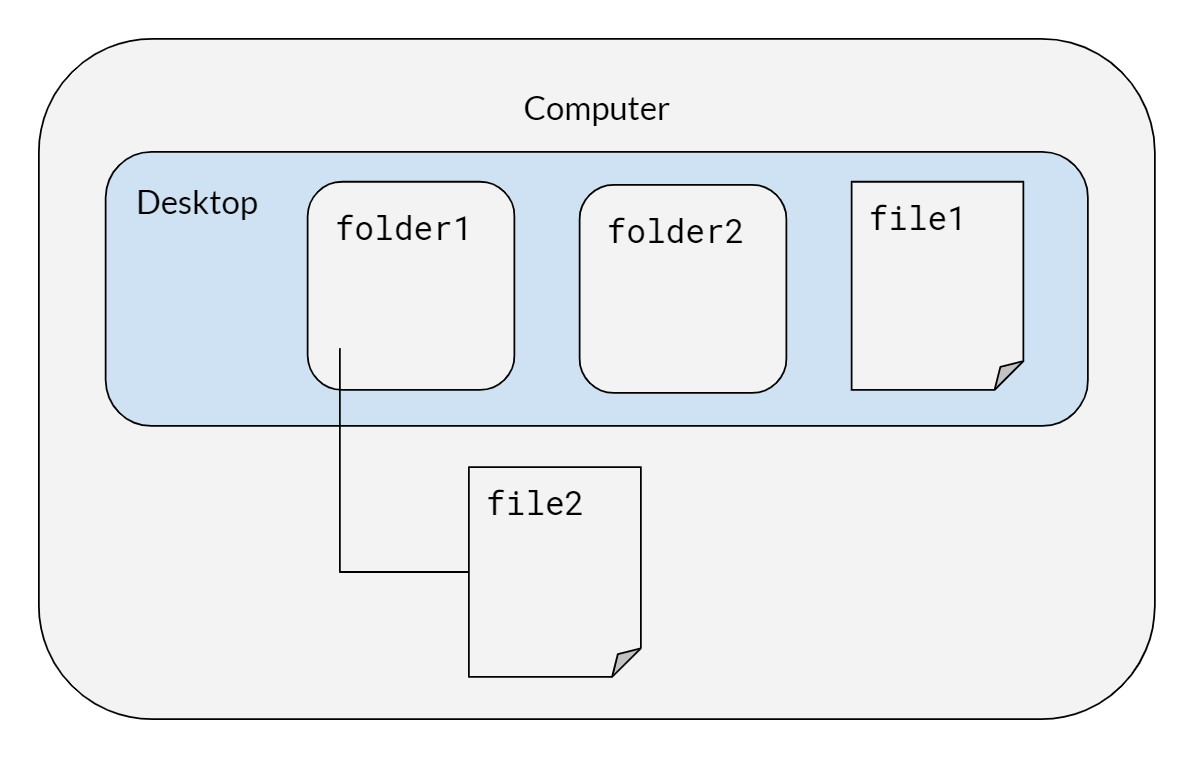
\includegraphics{assets/images/ex-desktop.jpg}
\caption{Here is our example desktop.}
\end{figure}

\hypertarget{syntax-for-both-macwindows}{%
\section{Syntax for both Mac/Windows}\label{syntax-for-both-macwindows}}

When typing in directories or file names, quotes are necessary if the name includes spaces.

\begin{longtable}[]{@{}
  >{\raggedright\arraybackslash}p{(\columnwidth - 2\tabcolsep) * \real{0.43}}
  >{\raggedright\arraybackslash}p{(\columnwidth - 2\tabcolsep) * \real{0.57}}@{}}
\toprule
Command & Description \\
\midrule
\endhead
\texttt{cd\ desktop/folder1} & Change directory to \texttt{folder1} \\
\texttt{pwd} & Print working directory \\
\texttt{ls} & List files in the directory \\
\texttt{cp\ "file2"\ "newfile2"} & Copy file (remember to include file extensions when typing in file names like \texttt{.pdf} or \texttt{.R}) \\
\texttt{mv\ “newfile2”\ “file3”} & Rename \texttt{newfile2} to \texttt{file3} \\
\texttt{cd\ ..} & Go to parent of the working directory (in this case, \texttt{desktop}) \\
\texttt{mv\ “file1”\ folder2} & Move \texttt{file1} to \texttt{folder2} \\
\texttt{mkdir\ folder3} & Make a new folder in \texttt{folder2} \\
\texttt{rm\ \textless{}filename\textgreater{}} & Remove files \\
\texttt{rm\ -rf\ folder3} & Remove directories (\texttt{-r} will attempt to remove the directory recursively, \texttt{-rf} will force removal of the directory) \\
\texttt{clear} & Clear terminal screen of all previous commands \\
\bottomrule
\end{longtable}

\begin{figure}
\centering
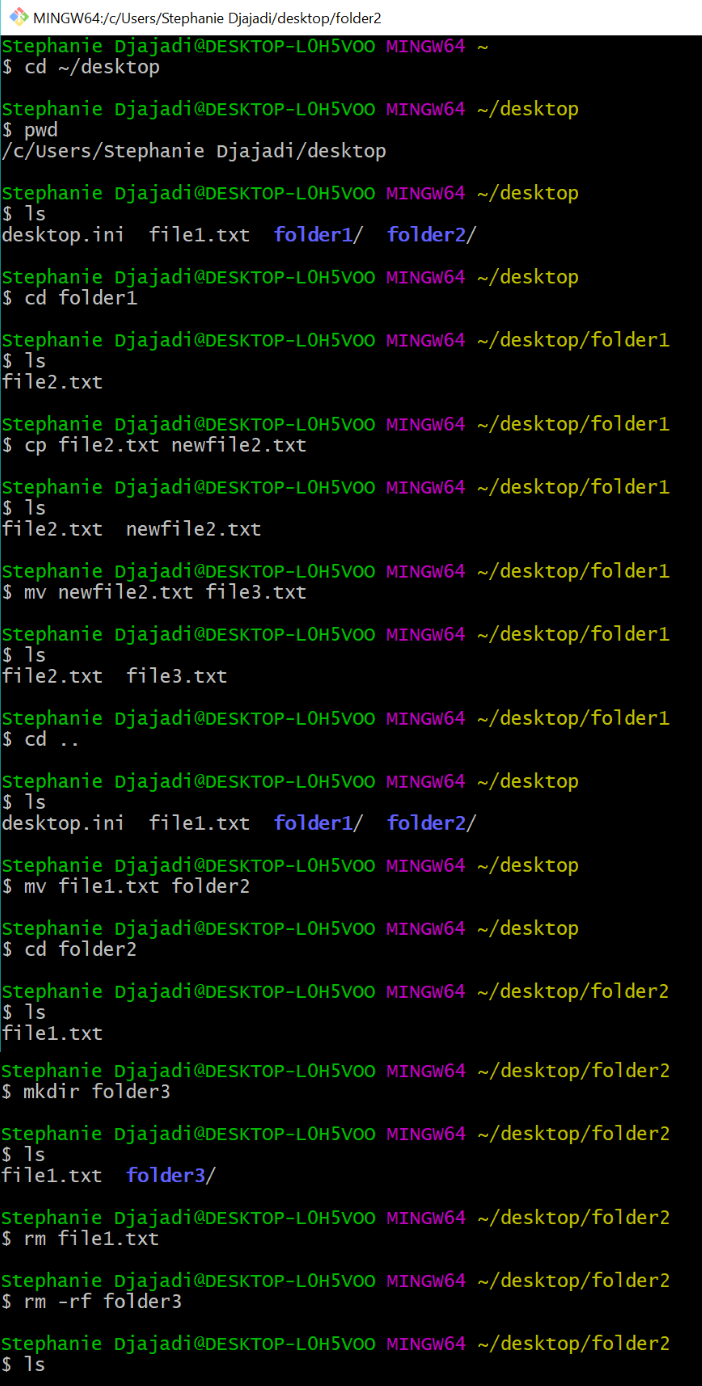
\includegraphics{assets/images/ex-terminal.PNG}
\caption{Here is an example of what your terminal might look like after executing the commands in the order listed above.}
\end{figure}

\hypertarget{running-bash-scripts}{%
\section{Running Bash Scripts}\label{running-bash-scripts}}

\begin{longtable}[]{@{}
  >{\raggedright\arraybackslash}p{(\columnwidth - 4\tabcolsep) * \real{0.26}}
  >{\raggedright\arraybackslash}p{(\columnwidth - 4\tabcolsep) * \real{0.37}}
  >{\raggedright\arraybackslash}p{(\columnwidth - 4\tabcolsep) * \real{0.37}}@{}}
\toprule
Windows & Mac / Linux & Description \\
\midrule
\endhead
\texttt{chmod\ +750\ \textless{}filename.sh\textgreater{}} & \texttt{chmod\ +x\ \textless{}filename.sh\textgreater{}} & Change access permissions for a file (only needs to be done once) \\
\texttt{./\textless{}filename.sh\textgreater{}} & \texttt{./\textless{}filename.sh\textgreater{}} & Run file (\texttt{./} to run any executable file) \\
\texttt{bash\ bash\_script\_name.sh\ \&} & \texttt{bash\ bash\_script\_name.sh\ \&} & Run shell script in the background \\
\bottomrule
\end{longtable}

\hypertarget{running-rscripts-in-windows}{%
\section{Running Rscripts in Windows}\label{running-rscripts-in-windows}}

\textbf{Note: This code seems to work only with Windows Command Prompt, not with Git Bash.}

When R is installed, it comes with a utility called Rscript. This allows you to run R commands from the command line. If Rscript is in your \texttt{PATH,} then typing Rscript into the command line, and pressing enter, will not error. Otherwise, to use Rscript, you will either need to add it to your PATH (as an environment variable), or append the full directory of the location of Rscript on your machine. To find the full directory, search for where R is installed your computer. For instance, it may be something like below (this will vary depending on what version of R you have installed):

\texttt{C:\textbackslash{}Program\ Files\textbackslash{}R\textbackslash{}R-3.6.0\textbackslash{}bin}

For appending the \texttt{PATH} variable, please view \href{https://www.howtogeek.com/118594/how-to-edit-your-system-path-for-easy-command-line-access/}{this link}. I strongly recommend completing this option.

If you add the PATH as an environment variable, then you can run this line of code to test:
\texttt{Rscript\ -e\ “cat(‘this\ is\ a\ test’)"}, where the \texttt{-e} flag refers to the expression that will be executed.

If you do not add the PATH as an environment variable, then you can run this line of code to replicate the results from above:
\texttt{“C:\textbackslash{}Program\ Files\textbackslash{}R\textbackslash{}R-3.6.0\textbackslash{}bin”\ -e\ “cat(‘this\ is\ a\ test’)”}

To run an R script from the command line, we can say:
\texttt{Rscript\ -e\ “source(‘C:/path/to/script/some\_code.R’)”}

\hypertarget{common-mistakes}{%
\subsection{Common Mistakes}\label{common-mistakes}}

\begin{itemize}
\tightlist
\item
  Remember to include all of the quotation marks around file paths that have a spaces.
\item
  If you attempt to run an R script but run into \texttt{Error:\ \textquotesingle{}\textbackslash{}U\textquotesingle{}\ used\ without\ hex\ digits\ in\ character\ string\ starting\ "\textquotesingle{}C:\textbackslash{}U"}, try replacing all \texttt{\textbackslash{}} with \texttt{\textbackslash{}\textbackslash{}} or \texttt{/}.
\end{itemize}

\hypertarget{checking-tasks-and-killing-jobs}{%
\section{Checking tasks and killing jobs}\label{checking-tasks-and-killing-jobs}}

\begin{longtable}[]{@{}
  >{\raggedright\arraybackslash}p{(\columnwidth - 4\tabcolsep) * \real{0.26}}
  >{\raggedright\arraybackslash}p{(\columnwidth - 4\tabcolsep) * \real{0.37}}
  >{\raggedright\arraybackslash}p{(\columnwidth - 4\tabcolsep) * \real{0.37}}@{}}
\toprule
Windows & Mac / Linux & Description \\
\midrule
\endhead
\texttt{tasklist} & \texttt{ps\ -v} & List all processes on the command line \\
& \texttt{top\ -o\ {[}cpu/rsize{]}} & List all running processes, sorted by CPU or memory usage \\
\texttt{taskkill\ /F\ /PID\ pid\_number} & \texttt{kill\ \textless{}PID\_number\textgreater{}} & Kill a process by its process ID \\
\texttt{taskkill\ /IM\ "process\ name"\ /F} & & Kill a process by its name \\
\texttt{start\ /b\ program.exe} & & Runs jobs in the background (exclude \texttt{/b} if you want the program to run in a new console) \\
& \texttt{nohup} & Prevents jobs from stopping \\
& \texttt{disown} & Keeps jobs running in the background even if you close R \\
\texttt{taskkill\ /?} & & Help, lists out other commands \\
\bottomrule
\end{longtable}

To kill a task in Windows, you can also go to Task Manager \textgreater{} More details \textgreater{} Select your desired app \textgreater{} Click on End Task.

\hypertarget{running-big-jobs}{%
\section{Running big jobs}\label{running-big-jobs}}

For big data workflows, the concept of ``backgrounding'' a bash script allows you to start a ``job'' (i.e.~run the script) and leave it overnight to run. At the top level, a bash script (\texttt{0-run-project.sh}) that simply calls the directory-level bash scripts (i.e.~\texttt{0-prep-data.sh}, \texttt{0-run-analysis.sh}, \texttt{0-run-figures.sh}, etc.) is a powerful tool to rerun every script in your project. See the included example bash scripts for more details.

\begin{itemize}
\tightlist
\item
  \textbf{Running Bash Scripts in Background}: Running a long bash script is not trivial. Normally you would run a bash script by opening a terminal and typing something like \texttt{./run-project.sh}. But what if you leave your computer, log out of your server, or close the terminal? Normally, the bash script will exit and fail to complete. To run it in background, type \texttt{./run-project.sh\ \&;\ disown}. You can see the job running (and CPU utilization) with the command \texttt{top} or \texttt{ps\ -v} and check your memory with \texttt{free\ -h}.
\end{itemize}

Alternatively, to keep code running in the background even when an SSH connection is broken, you can use \texttt{tmux}. In terminal or gitbash follow the steps below. This \href{https://medium.com/@jeongwhanchoi/install-tmux-on-osx-and-basics-commands-for-beginners-be22520fd95e}{site} has useful tips on using \texttt{tmux}.

\begin{Shaded}
\begin{Highlighting}[]
\CommentTok{\# create a new tmux session called session\_name}
\ExtensionTok{tmux}\NormalTok{ new }\AttributeTok{{-}ssession\_name}

\CommentTok{\# run your job of interest}
\ExtensionTok{R}\NormalTok{ CMD BATCH myjob.R }\KeywordTok{\&} 
  
\CommentTok{\# check that it is running}
\FunctionTok{ps} \AttributeTok{{-}v}

\CommentTok{\# to exit the tmux session (Mac)}
\ExtensionTok{ctrl}\NormalTok{ + b }
\ExtensionTok{d}

\CommentTok{\# to reopen the tmux session to kill the job or }
\CommentTok{\# start another job}
\ExtensionTok{tmux}\NormalTok{ attach }\AttributeTok{{-}tsession\_name} 
\end{Highlighting}
\end{Shaded}

\begin{itemize}
\item
  \textbf{Deleting Previously Computed Results}: One helpful lesson we've learned is that your bash scripts should remove previous results (computed and saved by scripts run at a previous time) so that you never mix results from one run with a previous run. This can happen when an R script errors out before saving its result, and can be difficult to catch because your previously saved result exists (leading you to believe everything ran correctly).
\item
  \textbf{Ensuring Things Ran Correctly}: You should check the \texttt{.Rout} files generated by the R scripts run by your bash scripts for errors once things are run. A utility file is include in this repository, called \texttt{runFileSaveLogs}, and is used by the example bash scripts to\ldots{} run files and save the generated logs. It is an awesome utility and one I definitely recommend using. Before using \texttt{runFileSaveLogs}, it is necessary to put the file in the home working directory. For help and documentation, you can use the command \texttt{./runFileSaveLogs\ -h}. See example code and example usage for \texttt{runFileSaveLogs} below.
\end{itemize}

\hypertarget{example-code-for-runfilesavelogs}{%
\subsection{\texorpdfstring{Example code for \texttt{runfileSaveLogs}}{Example code for runfileSaveLogs}}\label{example-code-for-runfilesavelogs}}

\begin{Shaded}
\begin{Highlighting}[]
\CommentTok{\#!/usr/bin/env python3}
\CommentTok{\# Type "./runFileSaveLogs {-}h" for help}

\ImportTok{import}\NormalTok{ os}
\ImportTok{import}\NormalTok{ sys}
\ImportTok{import}\NormalTok{ argparse}
\ImportTok{import}\NormalTok{ getpass}
\ImportTok{import}\NormalTok{ datetime}
\ImportTok{import}\NormalTok{ shutil}
\ImportTok{import}\NormalTok{ glob}
\ImportTok{import}\NormalTok{ pathlib}

\CommentTok{\# Setting working directory to this script\textquotesingle{}s current directory}
\NormalTok{os.chdir(os.path.dirname(os.path.abspath(}\VariableTok{\_\_file\_\_}\NormalTok{)))}

\CommentTok{\# Setting up argument parser}
\NormalTok{parser }\OperatorTok{=}\NormalTok{ argparse.ArgumentParser(description}\OperatorTok{=}\StringTok{\textquotesingle{}Runs the argument R script(s) {-} in parallel if specified {-} and moves the subsequent generated .Rout log files to a timestamped directory.\textquotesingle{}}\NormalTok{)}

\CommentTok{\# Function ensuring that the file is valid}
\KeywordTok{def}\NormalTok{ is\_valid\_file(parser, arg):}
    \ControlFlowTok{if} \KeywordTok{not}\NormalTok{ os.path.exists(arg):}
\NormalTok{        parser.error(}\StringTok{"The file }\SpecialCharTok{\%s}\StringTok{ does not exist!"} \OperatorTok{\%}\NormalTok{ arg)}
    \ControlFlowTok{else}\NormalTok{:}
        \ControlFlowTok{return}\NormalTok{ arg}

\CommentTok{\# Function ensuring that the directory is valid}
\KeywordTok{def}\NormalTok{ is\_valid\_directory(parser, arg):}
    \ControlFlowTok{if} \KeywordTok{not}\NormalTok{ os.path.isdir(arg):}
\NormalTok{        parser.error(}\StringTok{"The specified path (}\SpecialCharTok{\%s}\StringTok{) is not a directory!"} \OperatorTok{\%}\NormalTok{ arg)}
    \ControlFlowTok{else}\NormalTok{:}
        \ControlFlowTok{return}\NormalTok{ arg}

\CommentTok{\# Additional arguments that can be added when running runFileSaveLogs}
\NormalTok{parser.add\_argument(}\StringTok{\textquotesingle{}{-}p\textquotesingle{}}\NormalTok{, }\StringTok{\textquotesingle{}{-}{-}parallel\textquotesingle{}}\NormalTok{, action}\OperatorTok{=}\StringTok{\textquotesingle{}store\_true\textquotesingle{}}\NormalTok{, }\BuiltInTok{help}\OperatorTok{=}\StringTok{"Runs the argument R scripts in parallel if specified"}\NormalTok{)}
\NormalTok{parser.add\_argument(}\StringTok{"{-}i"}\NormalTok{, }\StringTok{"{-}{-}identifier"}\NormalTok{, }\BuiltInTok{help}\OperatorTok{=}\StringTok{"Adds an identifier to the directory name where this is saved"}\NormalTok{)}
\NormalTok{parser.add\_argument(}\StringTok{\textquotesingle{}filenames\textquotesingle{}}\NormalTok{, nargs}\OperatorTok{=}\StringTok{\textquotesingle{}+\textquotesingle{}}\NormalTok{, }\BuiltInTok{type}\OperatorTok{=}\KeywordTok{lambda}\NormalTok{ x: is\_valid\_file(parser, x))}

\NormalTok{args }\OperatorTok{=}\NormalTok{ parser.parse\_args()}
\NormalTok{args\_dict }\OperatorTok{=} \BuiltInTok{vars}\NormalTok{(args)}

\BuiltInTok{print}\NormalTok{(args\_dict)}

\CommentTok{\# Run given R Scripts}
\ControlFlowTok{for}\NormalTok{ filename }\KeywordTok{in}\NormalTok{ args\_dict[}\StringTok{"filenames"}\NormalTok{]:}
\NormalTok{  system\_call }\OperatorTok{=} \StringTok{"R CMD BATCH"} \OperatorTok{+} \StringTok{" "} \OperatorTok{+}\NormalTok{ filename}
  \ControlFlowTok{if}\NormalTok{ args\_dict[}\StringTok{"parallel"}\NormalTok{]: }
\NormalTok{    system\_call }\OperatorTok{=} \StringTok{"nohup"} \OperatorTok{+} \StringTok{" "} \OperatorTok{+}\NormalTok{ system\_call }\OperatorTok{+} \StringTok{" \&"}

\NormalTok{  os.system(system\_call)}

\CommentTok{\# Create the directory (and any parents) of the log files}
\NormalTok{currentUser }\OperatorTok{=}\NormalTok{ getpass.getuser()}
\NormalTok{currentTime }\OperatorTok{=}\NormalTok{ datetime.datetime.now().strftime(}\StringTok{"\%Y{-}\%m{-}}\SpecialCharTok{\%d}\StringTok{ \%H:\%M:\%S"}\NormalTok{)}
\NormalTok{logDirPrefix }\OperatorTok{=} \StringTok{"/home/kaiserData/logs/"} \CommentTok{\# Change to the directory where the logs should be saved}
\NormalTok{logDir }\OperatorTok{=}\NormalTok{ logDirPrefix }\OperatorTok{+}\NormalTok{ currentTime }\OperatorTok{+} \StringTok{"{-}"} \OperatorTok{+}\NormalTok{ currentUser }

\CommentTok{\# If specified, adds the identifier to the filename of the log}
\ControlFlowTok{if}\NormalTok{ args.identifier }\KeywordTok{is} \KeywordTok{not} \VariableTok{None}\NormalTok{:}
\NormalTok{  logDir }\OperatorTok{+=} \StringTok{"{-}"} \OperatorTok{+}\NormalTok{ args.identifier}

\NormalTok{logDir }\OperatorTok{+=} \StringTok{"/"}

\NormalTok{pathlib.Path(logDir).mkdir(parents}\OperatorTok{=}\VariableTok{True}\NormalTok{, exist\_ok}\OperatorTok{=}\VariableTok{True}\NormalTok{)}

\CommentTok{\# Find and move all logs to this new directory}
\NormalTok{currentLogPaths }\OperatorTok{=}\NormalTok{ glob.glob(}\StringTok{\textquotesingle{}./*.Rout\textquotesingle{}}\NormalTok{)}

\ControlFlowTok{for}\NormalTok{ currentLogPath }\KeywordTok{in}\NormalTok{ currentLogPaths:}
\NormalTok{  filename }\OperatorTok{=}\NormalTok{ currentLogPath.split(}\StringTok{"/"}\NormalTok{)[}\OperatorTok{{-}}\DecValTok{1}\NormalTok{]}
\NormalTok{  shutil.move(currentLogPath, logDir }\OperatorTok{+}\NormalTok{ filename)}
\end{Highlighting}
\end{Shaded}

\hypertarget{example-usage-for-runfilesavelogs}{%
\subsection{\texorpdfstring{Example usage for \texttt{runfileSaveLogs}}{Example usage for runfileSaveLogs}}\label{example-usage-for-runfilesavelogs}}

This example bash script runs files and generates logs for five scripts in the \texttt{kaiserflu/3-figures} folder. Note that the \texttt{-i} flag is used as an identifier to add \texttt{figures} to the filename of each log.

\begin{Shaded}
\begin{Highlighting}[]
\CommentTok{\#!/bin/bash}

\CommentTok{\# Copy utility run script into this folder for concision in call}
\FunctionTok{cp}\NormalTok{ \textasciitilde{}/kaiserflu/runFileSaveLogs \textasciitilde{}/kaiserflu/3{-}figures/}

\CommentTok{\# Run folder scripts and produce output}
\BuiltInTok{cd}\NormalTok{ \textasciitilde{}/kaiserflu/3{-}figures/}
\ExtensionTok{./runFileSaveLogs} \AttributeTok{{-}i} \StringTok{"figures"} \DataTypeTok{\textbackslash{}}
\NormalTok{fig{-}mean{-}season{-}age.R }\DataTypeTok{\textbackslash{}}
\NormalTok{fig{-}monthly{-}rate.R }\DataTypeTok{\textbackslash{}}
\NormalTok{fig{-}point{-}estimates{-}combined.R }\DataTypeTok{\textbackslash{}}
\NormalTok{fig{-}point{-}estimates.R }\DataTypeTok{\textbackslash{}}
\NormalTok{fig{-}weekly{-}rate.R}

\CommentTok{\# Remove copied utility run script}
\FunctionTok{rm}\NormalTok{ runFileSaveLogs}
\end{Highlighting}
\end{Shaded}

\hypertarget{slurm}{%
\chapter{Slurm and cluster computing}\label{slurm}}

by Anna Nguyen, and Jade Benjamin-Chung

When you need to run a script that requires a large amount of RAM, large files, or that uses parallelization, you can use Sherlock, Stanford's computing cluster. Sherlock uses Slurm, an open source, scalable cluster management and job scheduling system for computing clusters. Jade can email Sherlock managers to get you an account. Please refer to the \href{https://www.sherlock.stanford.edu/docs/overview/introduction/}{Sherlock user guide} to learn about the system and how to use it. Below, we include a few tips specific to how we use Sherlock in our lab.

\hypertarget{getting-started}{%
\section{Getting started}\label{getting-started}}

To access Sherlock, in terminal, log in using the following syntax and replace ``USERNAME'' with your Stanford alias. You will be prompted to enter your Stanford password (the same one you use for your email and other accounts) and to complete two-factor authentication.

\begin{verbatim}
ssh USERNAME@login.sherlock.stanford.edu
\end{verbatim}

Once you log in, you can view the contents of your home directory in command line by entering \texttt{cd\ \$HOME}. You can create subfolders within this directory using the \texttt{mkdir} command. For example, you could make a ``code'' subdirectory and clone a Github repository there using the following code:

\begin{verbatim}
cd $HOME
mkdir code
git clone https://github.com/jadebc/covid19-infections.git
\end{verbatim}

\hypertarget{one-time-system-set-up}{%
\subsection{One-Time System Set-Up}\label{one-time-system-set-up}}

To keep the install packages consistent across different nodes, you will need to explicitly set the pathway to your R library directory.

Open your \texttt{\textasciitilde{}/.Renviron} file (\texttt{vi\ \textasciitilde{}/.Renviron}) and append the following line:

\emph{Note: Once you open the file using \texttt{vi\ {[}file\_name{]}}, you must press \texttt{i} (on Mac OS) or \texttt{Insert} (on Windows) to make edits. After you finish, hit \texttt{Esc} to exit editing mode and type \texttt{:wq} to save and close the file.}

\begin{Shaded}
\begin{Highlighting}[]
\VariableTok{R\_LIBS=}\NormalTok{\textasciitilde{}/R/x86\_64{-}pc{-}linux{-}gnu{-}library/4.0.2}
\end{Highlighting}
\end{Shaded}

Alternatively, run an R script with the following code on Sherlock:

\begin{verbatim}
r_environ_file_path = file.path(Sys.getenv("HOME"), ".Renviron")
if (!file.exists(r_environ_file_path)) file.create(r_environ_file_path)

cat("\nR_LIBS=~/R/x86_64-pc-linux-gnu-library/4.0.2",
    file = r_environ_file_path, sep = "\n", append = TRUE)
\end{verbatim}

To load packages that run off of C++, you'll need to set the correct compiler options in your R environment.

Open the Makevars file in Sherlock (\texttt{vi\ \textasciitilde{}/.R/Makevars}) and append the following lines

\begin{Shaded}
\begin{Highlighting}[]
\VariableTok{CXX14FLAGS=}\NormalTok{{-}O3 }\ExtensionTok{{-}march=native} \AttributeTok{{-}mtune}\OperatorTok{=}\NormalTok{native }\AttributeTok{{-}fPIC}
\VariableTok{CXX14=}\NormalTok{g++}
\end{Highlighting}
\end{Shaded}

Alternatively, create an R script with the following code, and run it on Sherlock:

\begin{verbatim}
dotR = file.path(Sys.getenv("HOME"), ".R")
if (!file.exists(dotR)) dir.create(dotR)

M = file.path(dotR, "Makevars")
if (!file.exists(M)) file.create(M)

cat("\nCXX14FLAGS=-O3 -march=native -mtune=native -fPIC",
    "CXX14=g++",
    file = M, sep = "\n", append = TRUE)
\end{verbatim}

\hypertarget{moving-files-to-sherlock}{%
\section{Moving files to Sherlock}\label{moving-files-to-sherlock}}

The \texttt{\$HOME} directory is a good place to store code and small test files (quota: 15 GB per user). Save large files to the \texttt{\$SCRATCH} directory (quota: 100 TB per user). On the \texttt{\$SCRATCH} directory, files that are not modified after 90 days are automatically deleted. For this reason, it's best to create a bash script that records the file transfer process for a given project. See example code below:

\begin{Shaded}
\begin{Highlighting}[]
\CommentTok{\# note: the following steps should be done from your local }
\CommentTok{\# (not after ssh{-}ing into sherlock)}

\CommentTok{\# securely transfer folders from Box to sherlock home directory}
\CommentTok{\# note: the {-}r option is for folders and is not needed for files}
\FunctionTok{scp} \AttributeTok{{-}r} \StringTok{"Box/malaria{-}project/folder{-}1/"}\NormalTok{ USERNAME@login.sherlock.stanford.edu:/home/users/USERNAME/}

\CommentTok{\# securely transfer folders from Box to your sherlock scratch directory}
\FunctionTok{scp} \AttributeTok{{-}r} \StringTok{"Box/malaria{-}project/folder{-}2/"}\NormalTok{ USERNAME@login.sherlock.stanford.edu:/scratch/users/USERNAME/}

\CommentTok{\# securely transfer folders from Box to our shared scratch directory}
\FunctionTok{scp} \AttributeTok{{-}r} \StringTok{"Box/malaria{-}project/folder{-}3/"}\NormalTok{ USERNAME@login.sherlock.stanford.edu:/scratch/group/jadebc/}
\end{Highlighting}
\end{Shaded}

\hypertarget{installing-packages-on-sherlock}{%
\section{Installing packages on Sherlock}\label{installing-packages-on-sherlock}}

When you begin working on Sherlock, you will most likely encounter problems with installing packages. There is a package installation \href{https://drive.google.com/file/d/1eybh4j_G-r3pMZBCVA4QHoWZBo_cW5zb/view}{file} explicitly written for Sherlock that you should run before testing any code and sourcing the configuration file. You should only have to do this once. Do not attempt to do this in the RStudio Server (see next section), as you will have to re-do it for every new session you open. Sherlock requires that you specify the repository where the package is downloaded from. You may also need to add an additional argument to prevent the packages from locking:

\begin{Shaded}
\begin{Highlighting}[]
\FunctionTok{install.packages}\NormalTok{(“pgirmess”, }\AttributeTok{repos=}\NormalTok{“http}\SpecialCharTok{:}\ErrorTok{//}\NormalTok{cran.us.ur}\SpecialCharTok{{-}}\NormalTok{project.org”, }\AttributeTok{INSTALL\_opts =}\NormalTok{ ‘—no}\SpecialCharTok{{-}}\NormalTok{lock’)}
\end{Highlighting}
\end{Shaded}

You may also get an error message because Sherlock has some package dependencies as ``modules.'' These modules should be loaded on the command line. For example, the lme4 package requires nloptr, and you may encounter problems installing nloptr and its dependencies, e.g.~cmake, normally. Instead, try loading the following modules on the command line before opening R:

\begin{Shaded}
\begin{Highlighting}[]
\ExtensionTok{module} \AttributeTok{{-}{-}force}\NormalTok{ purge }\CommentTok{\# remove any previously loaded modules}
\ExtensionTok{ml}\NormalTok{ load devel cmake}
\ExtensionTok{ml}\NormalTok{ math eigen}
\ExtensionTok{module}\NormalTok{ load physics gdal}
\ExtensionTok{module}\NormalTok{ load physics proj}

\ExtensionTok{module}\NormalTok{ load R/4.0.2 }\CommentTok{\# or version being used for your project}
\end{Highlighting}
\end{Shaded}

Figuring out the issues with some packages will require some trial and error. If you are still encountering problems installing a package, you may have to install other dependencies manually by reading through the error messages. However, you can also reach out to the Sherlock team for help. You can email them at (\href{mailto:srcc-support@stanford.edu}{\nolinkurl{srcc-support@stanford.edu}}). They also hold \href{https://jumpstartsrcc.sites.stanford.edu/events/series/sherlock-office-hours}{office hours}.

\hypertarget{testing-your-code}{%
\section{Testing your code}\label{testing-your-code}}

Both of the following ways to test code on Sherlock are recommended for making small changes, such as editing file paths and making sure the packages and source files load. You should write and test the functionality of your script locally, only testing on Sherlock once major bugs are out.

\hypertarget{the-command-line}{%
\subsection{The command line}\label{the-command-line}}

There are two main ways to explore and test code on Sherlock. The first way is best for users who are comfortable working on the command line and editing code in base R. Even if you are not comfortable yet, this is probably the better way because these commands will transfer between Sherlock and other cluster computers using Slurm.

Typically, you will want to initially test your scripts by initiating a development node using the command \texttt{sdev}. This will allocate a small amount of computing resources for 1 hour. You can access R via command line using the following code.

\begin{Shaded}
\begin{Highlighting}[]
\CommentTok{\# start development node}
\ExtensionTok{sdev}

\CommentTok{\# load R {-} default version (see Sherlock documentation for which version)*}
\ExtensionTok{module}\NormalTok{ load R}

\CommentTok{\# initiate R in command line}
\ExtensionTok{R}
\end{Highlighting}
\end{Shaded}

*Note: for collaboration purposes, it's best for everyone to work with one version of R. Check what versions others working on the project use. Some packages only work with some versions of R, so it's best to keep it consistent.

\hypertarget{the-sherlock-ondemand-dashboard}{%
\subsection{The Sherlock OnDemand Dashboard}\label{the-sherlock-ondemand-dashboard}}

The second way to test and edit code is to use the Sherlock OnDemand Dashboard, accessed by typing login.sherlock.stanford.edu into a web browser. You will be prompted to authenticate the way you would for any Stanford website. This is the best way for people who are not comfortable accessing \& editing in base R in a Shell application.

You can test your code via the \href{https://www.sherlock.stanford.edu/docs/user-guide/ondemand/\#rstudio}{Rstudio server on Sherlock}. Access this by clicking on Interactive Apps in the menu bar and choose R Studio Server. Similar to the sdev node, you have to set various parameters for your session. Choose a version of R and set the time -- max. 2 hours. You can play with the other configurations, but this is likely unnecessary, as you should not need huge computing power to test small amounts of code. Keep in mind the more computing power you request, the lower priority your request becomes. You will then wait for the resources to become available, and you will be able to click ``Launch'' when they are (if you don't mess with the CPU or GPU, this is usually less than 2 minutes). The screen that opens will look very similar to the RStudio on your local.

Do NOT use the RStudio Server's Terminal to install packages, set your R environment, and do everything else needed to configure Sherlock because you will likely need to re-do it for every session/project. It's best to use this if you are more comfortable testing \& editing in RStudio rather than through base R in a Shell application.

\hypertarget{filepaths-configuration-on-sherlock}{%
\subsection{Filepaths \& configuration on Sherlock}\label{filepaths-configuration-on-sherlock}}

In most cases, you will want to test that the file paths work correctly on Sherlock. You will likely need to add code to the configuration file in the project repository that specifies Sherlock-specific file paths. Here is an example:

\begin{Shaded}
\begin{Highlighting}[]
\CommentTok{\# set sherlock{-}specific file paths}
\ControlFlowTok{if}\KeywordTok{(}\ExtensionTok{Sys.getenv}\ErrorTok{(}\StringTok{"LMOD\_SYSHOST"}\KeywordTok{)}\ExtensionTok{==}\StringTok{"sherlock"}\KeywordTok{)\{}
  
  \ExtensionTok{sherlock\_path}\NormalTok{ = paste0}\ErrorTok{(}\ExtensionTok{Sys.getenv}\ErrorTok{(}\StringTok{"HOME"}\KeywordTok{)}\ExtensionTok{,} \StringTok{"/malaria{-}project/"}\KeywordTok{)}
  
  \ExtensionTok{data\_path}\NormalTok{ = paste0}\ErrorTok{(}\ExtensionTok{sherlock\_path,} \StringTok{"data/"}\KeywordTok{)}
  \ExtensionTok{results\_path}\NormalTok{ = paste0}\ErrorTok{(}\ExtensionTok{sherlock\_path,} \StringTok{"results/"}\KeywordTok{)}
\KeywordTok{\}}
\end{Highlighting}
\end{Shaded}

\hypertarget{running-big-jobs-1}{%
\section{Running big jobs}\label{running-big-jobs-1}}

Once your test scripts run successfully, you can submit an sbatch script for larger jobs. These are text files with a \texttt{.sh} suffix. Use a text editor like Sublime to create such a script. Documentation on sbatch options is available \href{https://slurm.schedmd.com/sbatch.html}{here}. Here is an example of an sbatch script with the following options:

\begin{itemize}
\tightlist
\item
  \texttt{job-name=run\_inc}: Job name that will show up in the Sherlock system
\item
  \texttt{begin=now}: Requests to start the job as soon as the requested resources are available
\item
  \texttt{dependency=singleton}: Jobs can begin after all previously launched jobs with the same name and user have ended.
\item
  \texttt{mail-type=ALL}: Receive all types of email notification (e.g., when job starts, fails, ends)
\item
  \texttt{cpus-per-task=16}: Request 16 processors per task. The default is one processor per task.
\item
  \texttt{mem=64G}: Request 64 GB memory per node.
\item
  \texttt{output=00-run\_inc\_log.out}: Create a log file called \texttt{00-run\_inc\_log.out} that contains information about the Slurm session
\item
  \texttt{time=47:59:00}: Set maximum run time to 47 hours and 59 minutes. If you don't include this option, Sherlock will automatically exit scripts after 2 hours of run time.
\end{itemize}

The file \texttt{analysis.out} will contain the log file for the R script \texttt{analysis.R}.

\begin{Shaded}
\begin{Highlighting}[]
\CommentTok{\#!/bin/bash}

\CommentTok{\#SBATCH {-}{-}job{-}name=run\_inc}
\CommentTok{\#SBATCH {-}{-}begin=now}
\CommentTok{\#SBATCH {-}{-}dependency=singleton}
\CommentTok{\#SBATCH {-}{-}mail{-}type=ALL}
\CommentTok{\#SBATCH {-}{-}cpus{-}per{-}task=16}
\CommentTok{\#SBATCH {-}{-}mem=64G}
\CommentTok{\#SBATCH {-}{-}mem=64G}
\CommentTok{\#SBATCH {-}{-}output=00{-}run\_inc\_log.out}
\CommentTok{\#SBATCH {-}{-}time=47:59:00}

\BuiltInTok{cd} \VariableTok{$HOME}\NormalTok{/malaria{-}code{-}repo/2{-}analysis/}

\ExtensionTok{module}\NormalTok{ purge }

\CommentTok{\# load R version 4.0.2 (required for certain packages)}
\ExtensionTok{module}\NormalTok{ load R/4.0.2}

\CommentTok{\# load gcc, a C++ compiler (required for certain packages)}
\ExtensionTok{module}\NormalTok{ load gcc/10}

\CommentTok{\# load software required for spatial analyses in R}
\ExtensionTok{module}\NormalTok{ load physics gdal}
\ExtensionTok{module}\NormalTok{ load physics proj}

\ExtensionTok{R}\NormalTok{ CMD BATCH }\AttributeTok{{-}{-}no{-}save}\NormalTok{ analysis.R analysis.out}
\end{Highlighting}
\end{Shaded}

To submit this job, save the code in the chunk above in a script called \texttt{myjob.sh} and then enter the following command into terminal:

\begin{Shaded}
\begin{Highlighting}[]
\ExtensionTok{sbatch}\NormalTok{ myjob.sh }
\end{Highlighting}
\end{Shaded}

To check on the status of your job, enter the following code into terminal:

\begin{Shaded}
\begin{Highlighting}[]
\ExtensionTok{squeue} \AttributeTok{{-}u} \VariableTok{$USERNAME}
\end{Highlighting}
\end{Shaded}

\hypertarget{checklists}{%
\chapter{Checklists}\label{checklists}}

by Jade Benjamin-Chung

\hypertarget{pre-analysis-plan-checklist}{%
\section{Pre-analysis plan checklist}\label{pre-analysis-plan-checklist}}

\begin{itemize}
\tightlist
\item
  Brief background on the study (a condensed version of the introduction section of the paper)
\item
  Hypotheses / objectives
\item
  Study design
\item
  Description of data
\item
  Definition of outcomes
\item
  Definition of interventions / exposures
\item
  Definition of covariates
\item
  Statistical power calculation
\item
  Statistical model description
\item
  Covariate selection / screening
\item
  Standard error estimation method
\item
  Missing data analysis
\item
  Assessment of effect modification / subgroup analyses
\item
  Sensitivity analyses
\item
  Negative control analyses
\end{itemize}

\hypertarget{code-checklist}{%
\section{Code checklist}\label{code-checklist}}

\begin{itemize}
\tightlist
\item
  Does the script run without errors?
\item
  Is code self-contained within repo and/or associated Box folder?
\item
  Is all commented out code / remarks removed?
\item
  Does the header accurately describe the process completed in the script?
\item
  Is the script pushed to its github repository?
\item
  Does the code adhere to the \href{https://jadebc.github.io/lab-manual/coding-style.html}{coding style guide}?
\item
  Are all warnings ignorable? Should any warnings be intentionally suppressed or addressed?
\end{itemize}

\hypertarget{manuscript-checklist}{%
\section{Manuscript checklist}\label{manuscript-checklist}}

\emph{This is adapted in part from \href{https://www.nature.com/articles/d41586-019-01431-z}{this article}.}

\begin{itemize}
\tightlist
\item
  Have you completed the relevant reporting checklist, if applicable? (\href{https://www.equator-network.org/about-us/what-is-a-reporting-guideline/}{Collection of checklists})
\item
  Are the study results within the manuscript replicable (i.e., if you rerun the code in the study's repository, the tables and figures will be exactly replicated?)
\item
  Is a target journal selected?
\item
  Is the title declarative, in other words, does it state the object/findings rather than suggest them?
\item
  Is the word count of the manuscript close to the target journal's allowance?
\item
  Does the manuscript adhere to the formatting guide of the target journal?
\item
  Does the manuscript use a consistent voice (passive or active -- usually active is preferred \ldots{} pun intended)?
\item
  Is each figure and table (including supplementary material) referenced in the main text?
\item
  Is there a caption for each figure and table (including supplementary material)?
\item
  Are tables/figures and supplementary material numbered in accordance with their appearance in the main text?
\item
  Does the text use past tense if it is reporting research findings or future tense if it is a study protocol?
\item
  Does the text avoid subjective wording (e.g., ``interesting'', ``dramatic'')?
\item
  Does the text use minimal abbreviations, and are all abbreviations defined at first use?
\item
  Does the text avoid directionless words? (e.g., instead of writing, `Precipitation influences disease risk', write, `Precipitation was associated with increased disease risk').
\item
  Does the text avoid making causal claims that are not supported by the study design? Be careful about the words ``effect'', ``increase'', and ``decrease'', which are often interpreted as causal.
\item
  Does the text avoid describing results with the word ``significant'', which can easily be confused with statistical significance? (see references on this topic \href{https://journals.lww.com/epidem/Fulltext/2001/05000/The_Value_of_P.2.aspx}{here})
\item
  Have you drafted author contributions? Do they follow the \href{https://journals.plos.org/plosone/s/authorship/?utm_source=plos\&utm_medium=blog\&utm_campaign=plos-1607-credit\#loc-author-contributions}{CRediT Taxonomy} for author contributions?
\end{itemize}

\hypertarget{figure-checklist}{%
\section{Figure checklist}\label{figure-checklist}}

\begin{itemize}
\tightlist
\item
  Are the x-axis and y-axis labeled?
\item
  If the figure includes panels, is each panel labeled?
\item
  Are there sufficient numerical / text labels and breaks on the x-axis and y-axis?
\item
  Is the font size appropriate (i.e., large enough to read, not so large that it distracts from the data presented in the figure?)
\item
  Are the colors used colorblind friendly? See a colorblind-friendly palette \href{http://www.cookbook-r.com/Graphs/Colors_(ggplot2)/\#a-colorblind-friendly-palette}{here}, a neat palette generator with colorblind options \href{https://medialab.github.io/iwanthue/?utm_source=Nature+Briefing\&utm_campaign=2c68711076-briefing-dy-20211006\&utm_medium=email\&utm_term=0_c9dfd39373-2c68711076-44335685}{here}, and an article on why this matters \href{https://www.nature.com/articles/d41586-021-02696-z}{here}
\item
  Are colors/shapes/line types defined in a legend?
\item
  Are the legends and other labels easy to understand with minimal abbreviations?
\item
  If there is overplotting, is transparency used to show overlapping data?
\item
  Are 95\% confidence intervals or other measures of precision shown, if applicable?
\end{itemize}

\hypertarget{resources}{%
\chapter{Resources}\label{resources}}

by Jade Benjamin-Chung and Kunal Mishra

\hypertarget{resources-for-r}{%
\section{Resources for R}\label{resources-for-r}}

\begin{itemize}
\tightlist
\item
  \href{https://www.rstudio.com/wp-content/uploads/2015/02/data-wrangling-cheatsheet.pdf}{dplyr and tidyr cheat sheet}
\item
  \href{https://www.rstudio.com/wp-content/uploads/2015/03/ggplot2-cheatsheet.pdf}{ggplot cheat sheet}
\item
  \href{https://s3.amazonaws.com/assets.datacamp.com/blog_assets/datatable_Cheat_Sheet_R.pdf}{data table cheat sheet}
\item
  \href{https://www.rstudio.com/wp-content/uploads/2015/02/rmarkdown-cheatsheet.pdf}{RMarkdown cheat sheet}
\item
  \href{http://adv-r.had.co.nz/Style.html}{Hadley Wickham's R Style Guide}
\item
  \href{https://ucb-epi-r.github.io}{Jade's R-for-epi course}
\item
  \href{https://www.youtube.com/watch?v=nERXS3ssntw}{Tidy Eval in 5 Minutes} (video)
\item
  \href{https://tidyeval.tidyverse.org/index.html}{Tidy Evaluation} (e-book)
\item
  \href{https://www.brodrigues.co/blog/2016-07-18-data-frame-columns-as-arguments-to-dplyr-functions/}{Data Frame Columns as Arguments to Dplyr Functions} (blog)
\item
  \href{https://stackoverflow.com/questions/28125816/r-standard-evaluation-for-join-dplyr}{Standard Evaluation for *\_join} (stackoverflow)
\item
  \href{https://dplyr.tidyverse.org/articles/programming.html}{Programming with dplyr} (package vignette)
\end{itemize}

\hypertarget{resources-for-git-github}{%
\section{Resources for Git \& Github}\label{resources-for-git-github}}

\begin{itemize}
\tightlist
\item
  \href{https://www.datacamp.com/courses/introduction-to-git-for-data-science}{Data Camp introduction to Git}
\item
  \href{https://lab.github.com/githubtraining/introduction-to-github}{Introduction to Github}
\end{itemize}

\hypertarget{scientific-figures}{%
\section{Scientific figures}\label{scientific-figures}}

\begin{itemize}
\tightlist
\item
  \href{https://journals.plos.org/ploscompbiol/article?id=10.1371/journal.pcbi.1003833}{Ten Simple Rules for Better Figures}
\end{itemize}

\hypertarget{writing}{%
\section{Writing}\label{writing}}

\begin{itemize}
\tightlist
\item
  \href{https://www.nature.com/articles/d41586-019-02918-5}{Tips on how to write a great science paper}
\item
  \href{http://www.icmje.org/recommendations/browse/roles-and-responsibilities/defining-the-role-of-authors-and-contributors.html}{ICMJE Definition of authorship}
\item
  \href{https://www.nature.com/articles/nphys724}{Nature article on elements of style for scientific writing}
\end{itemize}

\hypertarget{presentations}{%
\section{Presentations}\label{presentations}}

\begin{itemize}
\tightlist
\item
  \href{https://www.nature.com/articles/d41586-021-03603-2}{How to tell a compelling story in scientific presentations}
\end{itemize}

  \bibliography{book.bib,packages.bib}

\end{document}
